%\VignetteIndexEntry{Prostar user manual}
%\VignetteKeywords{MassSpectrometry, Proteomics, DAPAR}
%\VignettePackage{Prostar}


\documentclass[12pt]{article}
\usepackage{soul,color,colortbl}
\usepackage{url}
\usepackage[utf8]{inputenc}

\newcommand{\shellcmd}[1]{\\\indent\indent\texttt{\footnotesize\# #1}}
\newcommand{\bordurefigure}[1]{\fbox{\includegraphics{#1}}}

% to uncomment for R, to comment for LaTeX
\RequirePackage[]{C:/Users/EF249002/Documents/R/R-devel/library/BiocStyle/resources/tex/Bioconductor}
\AtBeginDocument{\bibliographystyle{C:/Users/EF249002/Documents/R/R-devel/library/BiocStyle/resources/tex/unsrturl}}
\usepackage[noae, nogin]{Sweave}

% to comment for R, to uncomment for LaTeX
%\RequirePackage[]{C:/Users/tb232477/Documents/R/R-3.5.1/library/BiocStyle/resources/tex/Bioconductor}


% to replace
\bioctitle{\Biocpkg{Prostar} user manual}
%\title{\Biocpkg{Prostar} user manual}

\author[1,$\ast$]{Samuel Wieczorek}
\author[1,2,$\ast$]{Thomas Burger}
\affil[1]{Univ. Grenoble Alpes, CEA, INSERM, BIG-BGE, 38000 Grenoble, France}
\affil[2]{CNRS, BIG-BGE, F-38000 Grenoble, France}
\affil[$\ast$]{\email{firstname.lastname@cea.fr}}

\usepackage{Sweave}
\begin{document}

% to uncomment for R, to comment for LaTeX
\Sconcordance{concordance:Prostar_UserManual.tex:Prostar_UserManual.Rnw:%
1 12 1 1 2 1 0 1 2 22 1 1 0 128 1 1 2 1 0 1 1 3 0 1 2 6 1 1 2 1 0 1 1 3 %
0 1 2 16 1 1 2 4 0 1 2 32 1 1 2 1 0 1 1 3 0 1 2 18 1 1 2 1 0 1 1 3 0 1 %
2 80 1 1 2 4 0 1 2 334 1 1 2 4 0 1 2 720 1 1 2 1 0 1 1 3 0 1 2 105 1 1 %
2 13 0 1 2 4 1}


\maketitle
%%%%%%%%%%%%%%%%%%%%%%%%%%%%%%%%%%%%%%%%%%%%%%%%%%%%%%%
%%%%%%%%%%%%%%%%%%%%%%%%%%%%%%%%%%%%%%%%%%%%%%%%%%%%%%%
%%%%%%%%%%%%%%%%%%%%%%%%%%%%%%%%%%%%%%%%%%%%%%%%%%%%%%%
%%%%%%%%%%%%%%%%%%%%%%%%%%%%%%%%%%%%%%%%%%%%%%%%%%%%%%%
%%%%%%%%%%%%%%%%%%%%%%%%%%%%%%%%%%%%%%%%%%%%%%%%%%%%%%%
%%%%%%%%%%%%%%%%%%%%%%%%%%%%%%%%%%%%%%%%%%%%%%%%%%%%%%%
%%%%%%%%%%%%%%%%%%%%%%%%%%%%%%%%%%%%%%%%%%%%%%%%%%%%%%%
%%%%%%%%%%%%%%%%%%%%%%%%%%%%%%%%%%%%%%%%%%%%%%%%%%%%%%%
%%%%%%%%%%%%%%%%%%%%%%%%%%%%%%%%%%%%%%%%%%%%%%%%%%%%%%%


%% Abstract and keywords %%%%%%%%%%%%%%%%%%%%%%%%%%%%%%%%
\vskip 0.3in minus 0.1in
\hrule
\begin{abstract}
\Biocpkg{Prostar} (Proteomics statistical analysis with R)
is a Bioconductor distributed R package which provides all the necessary 
functions to analyze quantitative data from label-free proteomics 
experiments. Contrarily to most other similar R packages, it is endowed
with rich and user-friendly graphical interfaces, so that no programming 
skill is required. This document covers the functionalities available 
in Prostar 1.19.11.
\end{abstract}
\packageVersion{Prostar 1.19.11; DAPAR 1.19.13; DAPARdata 1.17.0}
\vskip 0.1in minus 0.05in
\hrule
\vskip 0.2in minus 0.1in
%%%%%%%%%%%%%%%%%%%%%%%%%%%%%%%%%%%%%%%%%%%%%%%%%%%%%%%%%%

\newpage
\tableofcontents
\newpage

%%%%%%%%%%%%%%%%%%%%%%%%%%%%%%%%%%%%%%%%%%%%%%%%%%%%%%%%%%%%%%%%%%%%%%%%%%%%%%
\section{Introduction}\label{sec:intro}




\Biocpkg{DAPAR} and \Biocpkg{Prostar} are a series of software dedicated to 
the processing of proteomics data. More precisely, they are devoted to the 
analysis of quantitative datasets produced by bottom-up discovery proteomics 
experiments with a LC-MS/MS pipeline (Liquid Chromatography and Tandem Mass 
spectrometry).
\Biocpkg{DAPAR} (Differential Analysis of Protein Abundance with R) is an R 
package that contains all the necessary functions to process the data in 
command lines. It can be used on its own; or as a complement to the numerous 
Bioconductor packages (\url{https://www.bioconductor.org/}) it is compliant with; 
or through the \Biocpkg{Prostar} interface.
\Biocpkg{Prostar} (Proteomics statistical analysis with R) is a 
web interface based on Shiny technology (\url{http://shiny.rstudio.com/}) that provides GUI 
(Graphical User Interfaces)
to all the \Biocpkg{DAPAR} functionalities, so as to guide any 
practitioner that is not comfortable with R programming through the complete 
quantitative analysis process.
 The experiment package \Biocpkg{DAPARdata} contains 
many datasets that can be used as examples.
\Biocpkg{Prostar} functionalities make it possible to easily:
\begin{itemize}
\item \textbf{Manage quantitative datasets}\footnote{Here, a quantitative dataset 
denotes a table where each analyte (either a peptide or a protein) is represented
by a line and each replicate (or sample) is represented by a column; 
each cell of the table contains the abundance of a given analyte in a given replicate; 
the replicates are clustered into different conditions (or groups).}: This includes
import/export, conversion and report generation functionalities.
\item \textbf{Perform a complete data processing chain}: (\emph{i}) filtering and data cleaning; 
(\emph{ii}) cross-replicate normalization; (\emph{iii}) missing value imputation; (\emph{iv}) aggregation of peptide 
intensities into protein intensities (optional); (\emph{v}) null hypothesis significance testing.
\item \textbf{Mine the dataset} at any step of the processing chain with various tools such as:
(\emph{i}) descriptive statistics; (\emph{ii}) differential analysis; (\emph{iii}) Gene Ontology (GO) analysis.
\end{itemize}


%%%%%%%%%%%%%%%%%%%%%%%%%%%%%%%%%%%%%%%%%%%%%%%%%%%%%%%%%%%%%%%%%%%%%%%%%%%%%
%%%%%%%%%%%%%%%%%%%%%%%%%%%%%%%%%%%%%%%%%%%%%%%%%%%%%%%%%%%%%%%%%%%%%%%%%%%%%
%%%%%%%%%%%%%%%%%%%%%%%%%%%%%%%%%%%%%%%%%%%%%%%%%%%%%%%%%%%%%%%%%%%%%%%%%%%%%
\section{Installation}\label{sec:install}

There are many ways to install \Biocpkg{Prostar}, as well as its dependencies\footnote{i.e. Packages
that are necessary for \Biocpkg{Prostar} to correctly run.}:
\begin{enumerate}
	\item \textbf{Zero-install}: The easiest way, so far only available on Microsoft Windows desktop machines.
	\item \textbf{Stand-alone Bioconductor install}: The standard method to install Bioconductor distributed software. 
	This method works for any operating systems (Unix/Linux, Mac OS X and Windows) as long as R is installed.
	\item \textbf{Server install}: When one wants \Biocpkg{Prostar} to run on a Unix server, on which remote users connect.
\end{enumerate}
In addition, it is also possible to only install \Biocpkg{DAPAR} or \Biocpkg{DAPARdata},
so as to work in command lines (for expert users only).

For all the desktop installs, we advise to use a machine with a minimum of 8GB of RAM (although there are no strict constraints).

\subsection{Zero-install}
This method works for any desktop machine with Microsoft Windows. It is not necessary to have R already installed.
Go to \url{http://www.prostar-proteomics.org} and click on Zero-install download (Prostar menu). Download the zip file and unzip it.
The unzipped folder contains an executable file which directly launches \Biocpkg{Prostar}. Notice that at the first launch,
an internet connection is necessary, so as to finish the install.

\subsection{Stand-alone Bioconductor install}\label{sec:daparProstarstandalone}

For this type of install, the operating system of the desktop machine can be of any type (Unix/Linux, Mac OS X or Windows).
However, it is necessary to have the latest version of R (see Section~\ref{sec:sessionInfo}) installed in a directory where the user has read/write permissions. 
Optionally, an IDE (integrated development environment) such as R Studio (\url{https://www.rstudio.com/}) may be useful to conveniently deal with the various R package installs.

To install \Biocpkg{Prostar}, enter in the R console the following instructions:
\begin{Schunk}
\begin{Sinput}
> install.packages("BiocManager")
> BiocManager::install("Prostar")
\end{Sinput}
\end{Schunk}

Then, the following packages should be successfully installed: \Biocpkg{MSnbase}, \CRANpkg{RColorBrewer}, stats, \Biocpkg{preprocessCore}, \CRANpkg{Cairo}, \CRANpkg{png}, \CRANpkg{lattice}, \CRANpkg{reshape2}, \CRANpkg{gplots}, \Biocpkg{pcaMethods}, \CRANpkg{ggplot2}, \Biocpkg{limma}, \CRANpkg{knitr}, \CRANpkg{tmvtnorm}, \CRANpkg{norm}, \Biocpkg{impute}, \CRANpkg{doParallel}, \CRANpkg{stringr}, parallel, \CRANpkg{foreach}, \CRANpkg{grDevices}, graphics, \CRANpkg{openxlsx}, \CRANpkg{utils}, \CRANpkg{cp4p}, \CRANpkg{scales}, \CRANpkg{Matrix}, \CRANpkg{vioplot}, \CRANpkg{imp4p}, \CRANpkg{imputeLCMD}, \CRANpkg{highcharter}, \Biocpkg{DAPARdata}, \Biocpkg{siggenes}, \Biocpkg{graph}, \CRANpkg{lme4}, \CRANpkg{readxl}, \Biocpkg{clusterProfiler}, \CRANpkg{dplyr}, \CRANpkg{tidyr}, \CRANpkg{tidyverse}, \Biocpkg{AnnotationDbi},  \Biocpkg{DAPAR}, \Githubpkg{jrowen/rhandsontable}, \CRANpkg{data.table}, \CRANpkg{shinyjs}, \CRANpkg{DT}, \CRANpkg{shiny}, \CRANpkg{shinyBS}, \CRANpkg{shinyAce}, \CRANpkg{htmlwidgets}, \CRANpkg{webshot}, \CRANpkg{R.utils}, \CRANpkg{shinythemes}, \CRANpkg{XML}, \CRANpkg{later}.

For a better experience, it is advised (but not mandatory) to install the development version of the following packages: DT and highcharter. To do so, install the devtools package and execute the following commands:
\begin{Schunk}
\begin{Sinput}
> devtools::install_github('rstudio/DT')
> devtools::install_github('jbkunst/highcharter')
\end{Sinput}
\end{Schunk}

Once the package is installed, to launch \Biocpkg{Prostar}, then enter:
\begin{Schunk}
\begin{Sinput}
> library(Prostar)
> Prostar()
\end{Sinput}
\end{Schunk}

A new window of the default web browser opens. 

\subsection{Server install} \label{sec:daparProstarserver}

In the case of several \Biocpkg{Prostar} users that are not 
confortable with R (programming or installing), it is best to have a single 
version of \Biocpkg{Prostar} running on a Shiny server 
installed on a Unix/Linux server. The users will use \Biocpkg{Prostar} through 
a web browser, exactly if it were locally installed, yet, a single install has 
to be administrated. In that case, \Biocpkg{DAPAR} has to be classically 
installed (see Section~\ref{sec:daparalone}), while on the other hand, the 
installation of \Biocpkg{Prostar} is slightly different.

Shiny Server (\url{https://github.com/rstudio/shiny-server}) is a server program that 
makes Shiny applications available over the web. If Shiny Server is not installed yet, 
follow Shiny installation instructions.

Once a Shiny server is available, first install \Biocpkg{Prostar} as described in 
Section~\ref{sec:daparProstarstandalone}, so as to have the dependencies 
installed.

Then, execute the following line to get the install directory of 
Prostar:

\begin{Schunk}
\begin{Sinput}
> installed.packages()["Prostar","LibPath"]
\end{Sinput}
\end{Schunk}

The result of this command is now referred as \emph{/path\_to\_Prostar}.

Change the owner of the Shiny Server directory and log as shiny
\shellcmd{sudo chown shiny /srv/shiny-server}
\shellcmd{sudo su shiny}


Create a directory named \Biocpkg{Prostar} in the Shiny Server directory with 
the user shiny as owner and then copy the Prostar files.

Create the directory for the shiny application 
\shellcmd{mkdir /srv/shiny-server/Prostar}

Copy the ProstarApp directory within the shiny-server directory
\shellcmd{sudo cp -r /path\_to\_Prostar/ProstarApp/ /srv/shiny-server/Prostar}

Change the owner of the Shiny Server directory
\shellcmd{sudo chown -R shiny /srv/shiny-server}

Give the following permissions to the www directory
\shellcmd{chmod 755 /srv/shiny-server/Prostar/www}


Check if the configuration file of Shiny Server is correct.
For more details, please visit 
\url{http://rstudio.github.io/shiny-server/latest/}.

Now, the application should be available via a web browser at 
http://\emph{servername}:\emph{port}/Prostar.


\subsection{\Biocpkg{DAPAR} and \Biocpkg{DAPARdata} (alone)}\label{sec:daparalone}

This type of install should only be performed by advanced R users/programmers, or by the admin of a server version of \Biocpkg{Prostar}.

To install the package \Biocpkg{DAPAR} from the source file with administrator 
rights, start R and enter:

\begin{Schunk}
\begin{Sinput}
> source("http://www.bioconductor.org/biocLite.R")
> biocLite("DAPAR")
\end{Sinput}
\end{Schunk}

This step will automatically install the following packages:
\begin{itemize}
\item {From the CRAN}: \CRANpkg{RColorBrewer}, \CRANpkg{Cairo}, \CRANpkg{png}, \CRANpkg{lattice}, \CRANpkg{reshape2}, \CRANpkg{gplots}, \Biocpkg{pcaMethods}, \CRANpkg{ggplot2},  \CRANpkg{knitr}, \CRANpkg{tmvtnorm}, \CRANpkg{norm}, \CRANpkg{doParallel}, \CRANpkg{stringr}, parallel, \CRANpkg{foreach}, \CRANpkg{grDevices}, graphics, \CRANpkg{openxlsx}, \CRANpkg{utils}, \CRANpkg{cp4p}, \CRANpkg{scales}, \CRANpkg{Matrix}, \CRANpkg{vioplot}, \CRANpkg{imp4p}, \CRANpkg{imputeLCMD}, \CRANpkg{lme4}, \CRANpkg{readxl},  \CRANpkg{dplyr}, \CRANpkg{tidyr}, \CRANpkg{tidyverse}, \CRANpkg{highcharter}, stats.
\item {From the Bioconductor}: \Biocpkg{MSnbase},  \Biocpkg{preprocessCore}, \Biocpkg{limma}, \Biocpkg{impute}, \Biocpkg{DAPARdata}, \Biocpkg{siggenes}, \Biocpkg{graph}, \Biocpkg{clusterProfiler}, \Biocpkg{AnnotationDbi},  \Biocpkg{DAPAR}.
\end{itemize}

\Biocpkg{DAPARdata} is automatically installed with \Biocpkg{Prostar} or \Biocpkg{DAPAR}. However, it is possible to install it alone. Then, it  follows 
the classical way for Bioconductor packages. In a R console, enter:
\begin{Schunk}
\begin{Sinput}
> source("http://www.bioconductor.org/biocLite.R")
> biocLite("DAPARdata")
\end{Sinput}
\end{Schunk}

%%%%%%%%%%%%%%%%%%%%%%%%%%%%%%%%%%%%%%%%%%%%%%%%%%%%%%%%%%%%%%%%%%%%%%%%%%%%%%
%%%%%%%%%%%%%%%%%%%%%%%%%%%%%%%%%%%%%%%%%%%%%%%%%%%%%%%%%%%%%%%%%%%%%%%%%%%%%%
%%%%%%%%%%%%%%%%%%%%%%%%%%%%%%%%%%%%%%%%%%%%%%%%%%%%%%%%%%%%%%%%%%%%%%%%%%%%%%

\section{Navigating through \Biocpkg{Prostar} interface}

\subsection{First contact with \Biocpkg{Prostar}}\label{sec:firstcontact}
%\subsubsection{Home screen overview}
Right after \Biocpkg{Prostar} being launched, the web page depicted in Figure~\ref{fig:fig1} shows up in the default browser (stand-alone install) or in a portable one (zero install).
So far, the navbar only contains 3 menus: Prostar, Data manager and Help. However, as soon as data are loaded in the software, new menus contextualy appear (see Section~\ref{sec:synopsis}).

\begin{figure}
	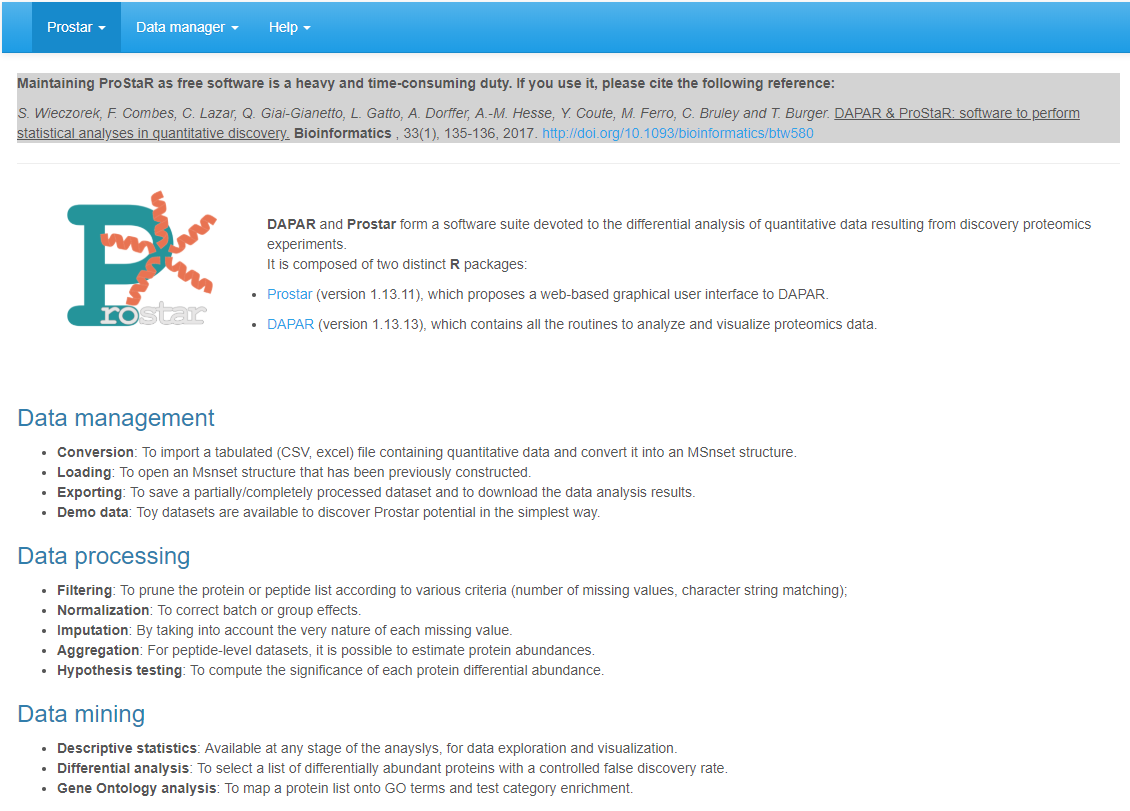
\includegraphics[width=\textwidth]{images/home.png}
	\caption{\Biocpkg{Prostar} home screen.}
	\label{fig:fig1}
\end{figure}

The \textbf{Data manager} is detailed in a dedicated section (Section~\ref{sec:manager}).  
%Here follows a brief description of  Prostar and Help menus, as well as some information on the data type and format.
%\subsubsection{Prostar menu}
In the \textbf{Prostar} menu, one has access to:
\begin{itemize}
	\item The \textbf{Home} screen\footnote{Going back to the home screen does not re-initialize the session.}, as illustrated on Figure~\ref{fig:fig1}.
	\item A \textbf{Global settings} menu, where it is possible to tune few parameters (such as colors, number of digits to display, etc.) that will affect the entire session.
	\item A page gathering \textbf{Release notes}, i.e. some information regarding the new features/changes/corrections with respect to the previous version.
	\item A \textbf{Check for updates} page, where it is possible to verify that the current version of \Biocpkg{Prostar} is not outdated.
\end{itemize}

%\subsubsection{Help menu}\label{sec:help}

In the \textbf{Help} menu, one has access to:
\begin{itemize}
	\item A list of \textbf{Useful links}: This page gather links towards numerous documents, such as scientific publications related to \Biocpkg{Prostar} as well as user manuals, reference manuals and tutorials.
	\item A series of frequently asked questions (\textbf{FAQ}) is also available. This page should be regularly visisted! %When facing any issue, any user is advised to check here first for an easy solution.
	\item A form screen to \textbf{Report a bug} (see below for details).
\end{itemize}

\Biocpkg{Prostar} is under active 
development, so that despite the developers' attention, bugs may remain. 
To signal any, as well as typos, suggestions, etc. or even to ask a question, 
please contact the developers. 

%\subsection{Understanding \Biocpkg{Prostar} interface}
\subsection{Synoptic view of \Biocpkg{Prostar} interface}\label{sec:synopsis}

When data are loaded for analysis, mor options are available in the navbar, as illustrated on Figure~\ref{fig:fig2}. In addition to the navbar, the screen is composed of a large working panel (below the navbar) and a drop-down menu on the upper right corner (which purpose is detailed in Section~\ref{sec:availabledatasets}).

\begin{figure}
		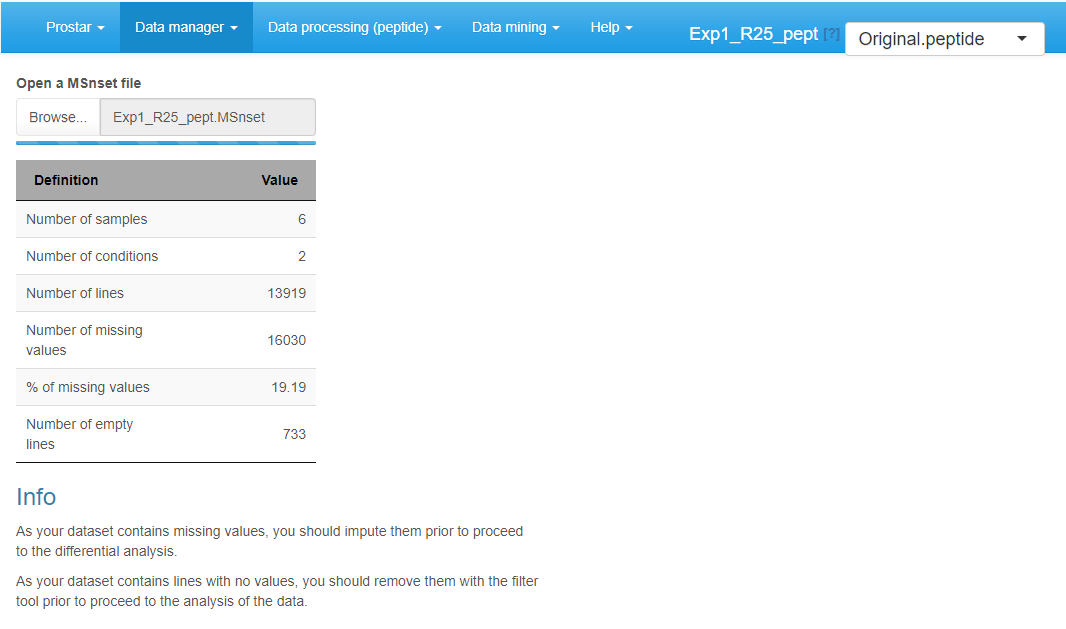
\includegraphics[width=1.00\textwidth]{images/load-pep.png}
	\caption{Screenshot illustrating the fully displayed navbar.}
	\label{fig:fig2}
\end{figure}

Table~\ref{tab:LoMenus} summarizes the content of the navbar. Let us note that depending on the dataset content (either proteins or peptides), the menu can slightly change: Notably, if protein-level dataset is loaded, then \textbf{Aggregation} (which purpose is to roll up from peptides to proteins) is not proposed in the \textbf{Data processing} menu.

\begin{table}
{\normalsize
		\begin{tabular}{|l|l|l|}
				\hline
		\cellcolor{black}\textbf{\textcolor[rgb]{1,1,1}{Prostar (\ref{sec:firstcontact})}} &	
		\cellcolor{black}\textbf{\textcolor[rgb]{1,1,1}{Data manager}} &	
		\cellcolor{black}\textbf{\textcolor[rgb]{1,1,1}{Data processing}} \\
		\hline
		Home &	Open MSnset file (\ref{sec:load}) &	Filter data (\ref{sec:filtering})  \\	
		Global settings	& Convert data (\ref{sec:import}) & Normalization (\ref{sec:normalization})  \\
		Release notes &	Demo data (\ref{sec:demomode}) &	Imputation (\ref{sec:imputation})  \\
		Check for updates & Export (\ref{sec:export}) &	Aggregation (\ref{aggregation})	 \\
		& &	Hypothesis testing (\ref{sec:hp})	 \\
		\hline
		\end{tabular} \newline \bigskip
		
	\begin{tabular}{|l|l|}
				\hline
		\cellcolor{black}\textbf{\textcolor[rgb]{1,1,1}{Data mining}}	& 
		\cellcolor{black}\textbf{\textcolor[rgb]{1,1,1}{Help (\ref{sec:firstcontact})}} \\
		\hline
		Descriptive statistics (\ref{sec:descriptivestatistics}) &	Useful links \\	
		Differential analysis (\ref{diffana}) &	FAQ \\
		GO analysis (\ref{sec:GOAnalysis}) &	Bug report\\
		\hline
		\end{tabular}
	}
	\caption{Synoptic view of the ProStaR menus with the corresponding reference sections.}
	\label{tab:LoMenus}
\end{table}

%\subsubsection{The ``Data manager'' menu}
The \textbf{Data manager} menu gathers all the functionalities that relates to data import, export or conversion:
\begin{itemize}
	\item \textbf{Open MSnset file} (see Section~\ref{sec:load}) should be used to reload a dataset that has previously been converted and saved as an MSnset object.
	\item \textbf{Convert data} (see Section~\ref{sec:import}) should be used to load a new dataset from a tabular file containing quantitative proteomics data, such as a Maxquant or Proline output.
	\item \textbf{Demo data} (see Section~\ref{sec:demomode}) makes it possible for any new user to discover \Biocpkg{Prostar} capabilities on toy datasets.
	\item \textbf{Export} (see Section~\ref{sec:export}) gathers all the functionalities to save a dataset in various formats, as well as to export the main results in a single document.
\end{itemize}
As soon as one of the three first options of the menu has been used to load a dataset, the \textbf{Data processing} and \textbf{Data mining} menus appear in the navbar.

%\subsubsection{The ``Data processing'' menu}
Conducting a rigorous differential analysis requires a well-defined pipeline made of several tightly connected steps. In \Biocpkg{Prostar}, this pipeline has been designed to be as general as possible. Thus, the \textbf{Data processing} menu contains numerous steps which, for a given dataset may not all be necessary, so that some can be occasionally skiped. However, the pipeline has been assembled and organized so as to propose coherent processing, so that the respective order of the different steps should be respected. These steps are the following:
\begin{enumerate}
	\item \textbf{Filtering} (see Section~\ref{sec:filtering}): to remove some analytes (because of too many missing values, or because they are irrelevent)
	\item \textbf{Normalization} (see Section~\ref{sec:normalization}): to correct batch effect and sample/condition biases
	\item \textbf{Imputation} (see Section~\ref{sec:imputation}): to impute the remaning missing values
	\item \textbf{Aggregation} (see Section~\ref{aggregation}): if the dataset is a peptide-level one, it is possible to aggregate them, so as to form a protein-level dataset
	\item \textbf{Hypothesis testing} (see Section~\ref{sec:hp}) of the differential abundance
\end{enumerate}
It should be carefully noted that each of these steps modifies the dataset: In other words, the \textbf{Data processing} menu offers a succession of data transformations which should be performed by the user in an educated way.

%\subsubsection{The ``Data mining'' menu}
As opposed to the \textbf{Data processing} menu, the \textbf{Data mining} menu offers a series of tools to analyze and visualize the dataset without transforming it. Thus, there is far less restriction on how and when applying them:
\begin{itemize}
	\item The \textbf{Descriptive statistics} (see Section~\ref{sec:descriptivestatistics}) panel is composed of several tabs which provide various ``static'' views on the dataset. It is advised to look at them between each processing step, so as to check how the dataset has been transformed.
	\item Once p-values have been computed (either at peptide or protein level) (see \textbf{Hypothesis testing} in the \textbf{Data processing} menu), it is possible to conduct a \textbf{Differential analysis} (see Section~\ref{diffana}). This consists in a series of statistical computations which purpose is to isolate a subset of proteins deemed differentially abundant between the compared conditions, according to a specific false discovery rate threshold.
	\item As long as the dataset is a protein-level one, it is possible to conduct a Gene Ontology (GO) enrichment or analysis on it (see Section~\ref{sec:GOAnalysis}). However, if the dataset is a peptide-level one, this option does not appear.
\end{itemize}

\subsection{Successive dataset versions}\label{sec:availabledatasets}

As explained above, each functionality in the \textbf{Data processing} menu transforms the current dataset.
To authorize some flexibility and to avoid unwanted data corruption, it is possible to save in \Biocpkg{Prostar} 
the original dataset, as well as each intermediate dataset along the processing chain. Concretely, it is possible
to store one ``original dataset'', one ``filtered dataset'', one ``normalized dataset'', one ``imputed dataset'' and so on.
Moreover, at any moment, it is possible to go back to a previous state of the dataset, either to restart a step that went wrong,
or just to compare with the \textbf{Data mining} tools how the dataset was changed (rapid switching makes it easier to visualize it).

To create a new item in the dataset history, one simply has to click on the save button at the end of each processing step. 
Each time a new dataset is  created, it is by default the one on which the processing goes on.

To navigate through the dataset history, one simply uses the drop-down menu of the upper right corner. Notice that 
if the user saves the current step (e.g.  
imputation), then goes back to a previous step (e.g. normalization 
) and start working on this older dataset (to perform
another imputation) and then saves it, the new version of the processing 
overwrites the previous version (the older imputation is lost and only the 
newest one is stored in memory): in fact, only a single version of the 
dataset can be saved for a given processing step. As a side effect, if any processing further than imputation was already done
(e.g. aggregation), then, the aggregated dataset is not coherent anymore with the imputed one (as the new imputation cannot be
automatically transmitted to update the previously tuned aggregation).

Finally, let us note that the name of each dataset version (normalized, imputed, etc.) also indicates if the dataset is a protein-level
or a peptide-level one (as for instance the aggregation step transforms a peptide-level dataset into a protein-level one).

\section{Data type and format}\label{sec:dataformat}
The quantitative data should fit into a matrix-like representation where each line corresponds to an analyte\footnote{The analytes can be either proteins or peptides. However, in a given dataset, all the analytes should be of the same nature.} and each column to a sample. Within the ($i$-th, $j$-th) cell of the matrix, one reads the abundance of analyte $i$ in sample $j$.

Although strictly speaking, there is no lower or upper bound to the number of lines, it should be recalled that the statistical tools implemented in \Biocpkg{Prostar} have been chosen and tuned to fit a discovery experiment dataset with large amount of analytes, so that the result may lack of reliability on too small datasets. Conversely, very large datasets are not inherently a problem, as R algorithms are well scalable, but one should keep in mind the hardware limitations of the machine on which \Biocpkg{Prostar} runs to avoid overloading. 

As for the number of samples (the columns of the dataset), it is necessary to have at least 2 conditions (or groups of samples) as it is not possible to perform relative comparison otherwise. Moreover, it is necessary to have at least 2 samples per condition\footnote{With only two replicates per conditions, the computations are tractable. It does not mean that statistical validity is guaranteed. 

Classically, 3 replicates per conditions are considered a minimum in case of a controlled experiment with a small variability, mainly issuing from technical or analytical repetitions. Analysis of complex proteomes between conditions with a large biological variability requires more replicates per conditions (5 to 10).}, as otherwise, it is not possible to compute an intra-condition variance, which is a prerequisite to numerous processing. 

The data table should be formatted in a tabulated file where the first line of the text file contains the column names. It is recommended to avoid special characters such as "]", "@", "\$", "\%", etc. that are automatically removed. Similarly, spaces in column names are replaced by dots ("."). Dot must be used as decimal separator for quantitative values. In addition to the columns containing quantitative values, the file may contain additional columns for metadata. Alternatively, if the data have already been processed by \Biocpkg{Prostar} and saved as an MSnset file (see \Biocpkg{MSnbase}), it is possible to directly reload them (see Section~\ref{sec:load}). 

%%%%%%%%%%%%%%%%%%%%%%%%%%%%%%%%%%%%%%%%%%%
%% Menu
%%%%%%%%%%%%%%%%%%%%%%%%%%%%%%%%%%%%%%%%%%%
\section{Data manager}\label{sec:manager}
The \textbf{Dataset manager} allows it to open, import or export quantitative 
datasets. \Biocpkg{Prostar} relies on the MSnSet format which 
is part of the package \Biocpkg{MSnbase}:
%~\cite{}.
It is either possible to load existing MSnSet files (see 
Section~\ref{sec:load}), or to import text (-tabulated) and Excel files (see 
Section~\ref{sec:import}). The \textbf{Demo data} menu allows it to load 
the datasets of the package \Biocpkg{DAPARdata} as examples to discover
\Biocpkg{Prostar} functionalities (see Section~\ref{sec:demomode}).


\subsection{Open MSnSet file} \label{sec:load}
To reload a dataset that was already formated into an MSnSet file, click
on \textbf{Open MSnset File}. This opens a 
pop-up window, so as to let the user choose the appropriate file. Once the 
file is uploaded, a short summary of the dataset is shown (see Figure~\ref{fig:fig2}): 
It includes the 
number of samples, the number of proteins (or peptides) in the dataset, the percentage of 
missing values and the number of lines which only contain missing 
values. Once done, the menu displaying the version of the dataset appears and display "Original - peptide" 
or "Original - protein", depending on whether the file contains peptide-level or
protein-level quantitative information (see Section~\ref{sec:availabledatasets}). 
Similarly, the Data processing and Data mining menus become available.

\subsection{Convert data}\label{sec:import}
To upload data from tabular file (i.e. stored in a file with one of the following extensions: .txt, .csv, .tsv, .xls, or .xlsx) click on the upper menu \textbf{Data manager} then chose \textbf{Convert data}. 

\textbf{First},  go to the \textbf{Select File} tab (see Figure~\ref{fig:imp1}): Click on the \textbf{Browse$\ldots$} button and select the tabular file of interest\footnote{The \Biocpkg{DAPARdata} package also contains tabular versions (in txt format) of the datasets available in the Demo data menu. Thus, it is also possible to test the import/export/save/load functions of \Biocpkg{Prostar} with these toy datasets. Concretely, one simply has to import them from the folder where the R packages are installed, in the following sub-folder: \texttt{.../R/R-3.4.0/library/DAPARdata/extdata}. Note that each dataset is also available in the MSnset format, but these datasets should not be considered to test conversion functions from/to tabular formats.} 
(If an Excel file is chosen, a drop-down menu appears to select the spreadsheet containing the data).
Once the upload is complete, indicate whether it is a protein level dataset (i.e., each line of the data table should correspond to a single protein) or a peptide-level one.
Indicate if the data are already log-transformed or not. If not they will be automatically log-transformed\footnote{\Biocpkg{Prostar} cannot process non-log-transformed data. Thus, do not cheat the software by indicating data on their original scale are log-transformed.}.
If the quantification software uses ``0'' in places of missing values, tick the last option ``Replace all 0 and NaN by NA'' (as in \Biocpkg{Prostar}, 0 is considered a value, not a missing value).
\begin {figure}
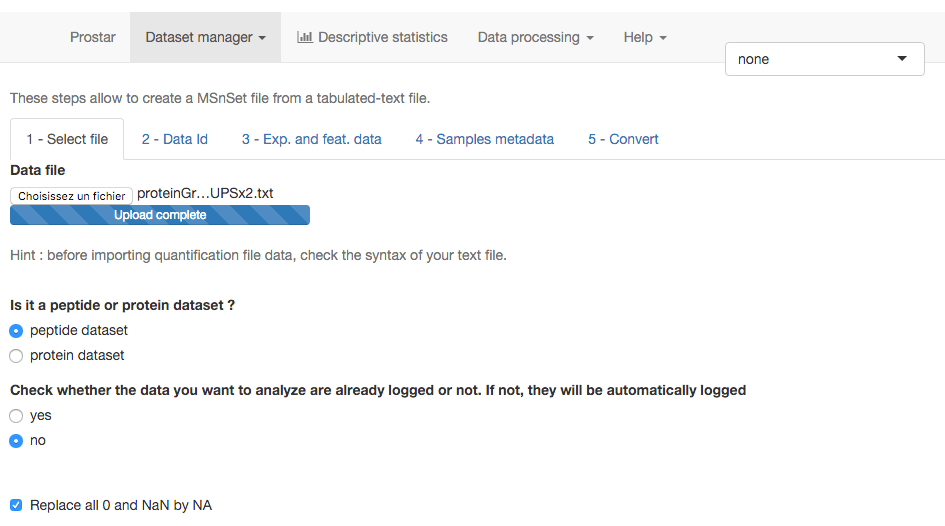
\includegraphics[width=\textwidth]{images/convert_selectfile.png}
\caption{File conversion, step 1.}\label{fig:imp1}
\end {figure}

\textbf{Second}, move on to the \textbf{Data Id} tab (see Figure~\ref{fig:imp2}): If the dataset already contains an ID column (a column where each cell has a unique content, which can serve as an ID for the peptides/proteins), select its name in the drop-down menu. Otherwise, it is possible to use the first option of the drop-down menu, that is the \textbf{Automatic ID definition}, which creates an artificial index. Finally, if the dataset is a peptide-level one, it is in addition important to indicate the column containing the IDs of the parent proteins, so as to prepare for future peptide to protein aggregation. 

\begin {figure}
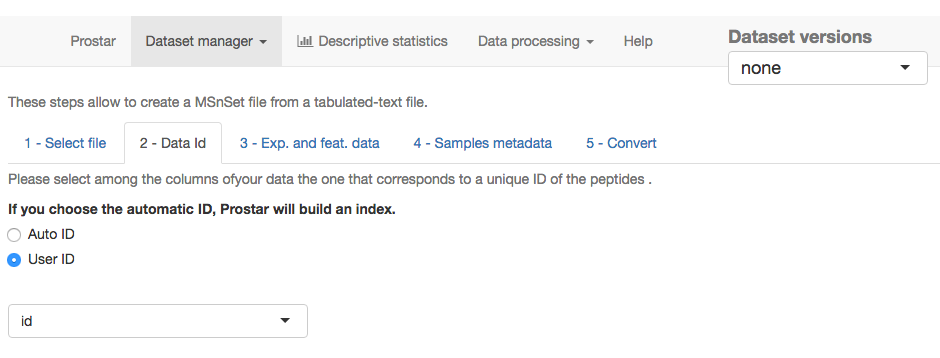
\includegraphics[width=\textwidth]{images/convert_dataID.png}
\caption{File conversion, step 2.}\label{fig:imp2}
\end {figure}

\textbf{On the third tab} (see Figure~\ref{fig:imp3}), referred to as \textbf{Exp. and feat. data},
select the columns which contain the protein abundances (one column for each sample of each condition). To select several column names in a row, click-on on the first one, and click-off on the last one. Alternatively, to select several names which are not continuously displayed, use the \textbf{Ctrl} key to maintain the selection.
If, for each sample, a column of the dataset provides information on the identification method (e.g. by direct MS/MS evidence, or by mapping) check the corresponding tick box. Then, for each sample, select the corresponding column. If none of these pieces of information is given, or, on the contrary, if all of them are specified with a different column name, a green logo appears, indicating it is possible to proceed (however, the content of the specified columns are not checked, so that it is the user's responsibility to select the correct ones). Otherwise (i.e. the identification method is given only for a subset of samples, or a same identification method is referenced for two different samples), then a red mark appears, indicating some corrections are mandatory.
\begin {figure}
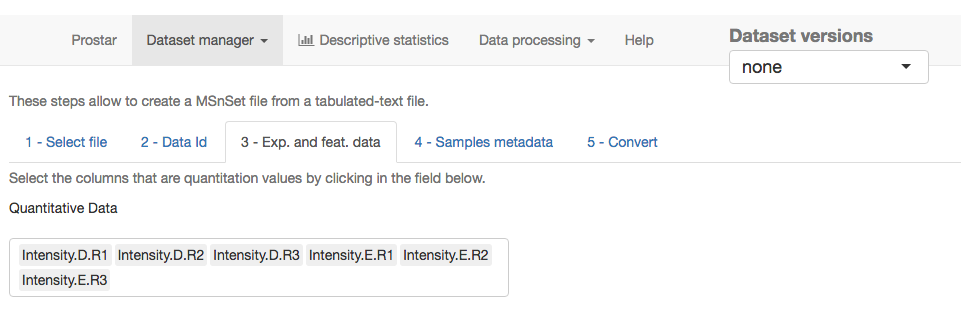
\includegraphics[width=\textwidth]{images/convert_exp_featdata.png}
\caption{File conversion, step 3.}\label{fig:imp3}
\end {figure}

\textbf{Move on to the fourth tab}, \textbf{Sample metadata} (see Figure~\ref{fig:imp4}). This tab guides the user through the definition of the experimental design.
Fill the empty columns with as different names as biological conditions to compare (minimum 2 conditions and 2 samples per condition) and click on \textbf{Check conditions}. If necessary, correct until the conditions are valid\footnote{As an help, it is possible to refer to FAQ \# 2}. When achieved, a green logo appears and the sample are reordered according to the conditions.
Choose the number of levels in the experimental design (either 1, 2 or 3), and fill the additional column(s) of the table\footnote{In case of difficulty, either to choose the adapted design hierarchy or to fill the table design, it is possible to click on the interrogation mark beside the sentence ``Choose the type of experimental design and complete it accordingly''. Except for flat design, which are automatically defined, it displays an example of the corresponding design. It is possible to rely on this example to precisely fill the design table.}.
Once the design is valid (a green check logo appears), move on to the last tab.

\begin {figure}
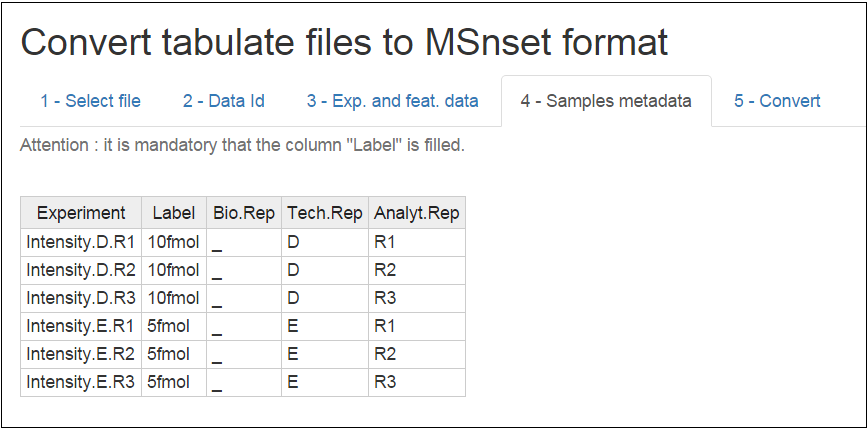
\includegraphics[width=\textwidth]{images/convert_sampledata.png}
\caption{File conversion, step 4.}\label{fig:imp4}
\end {figure}

\textbf{Finally}, move on to the \textbf{Convert} tab (see Figure~\ref{fig:imp5}).
Provide a name to the dataset to be created and click on the \textbf{Convert} button.
As a result, a new MSnset structure is created and automatically loaded. This can be checked with the name of the file appearing in the upper right hand side of the screen, as a title to a new drop-down menu. So far, it only contains ``Original - protein'' or ``Original - peptide'', but other versions of the dataset will be added along the course of the processing. Pay attention to any red message appears below the \textbf{Convert data} button, which indicates a mistake or an incomplete parameter tuning that must be sorted out before converting the data.
\begin {figure}
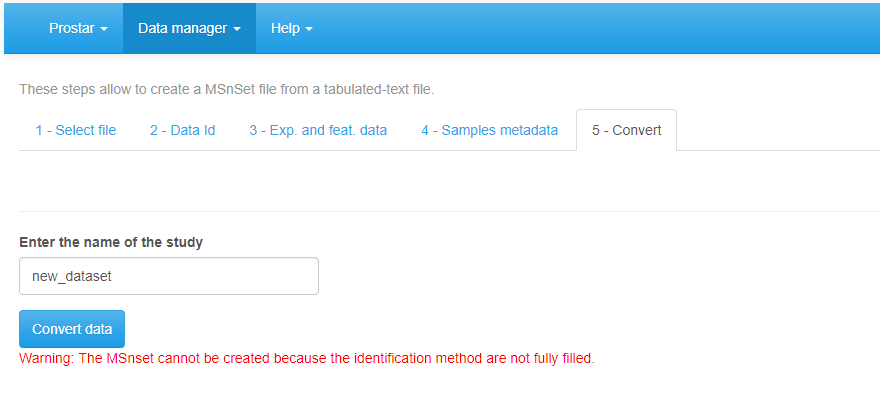
\includegraphics[width=\textwidth]{images/convert_convert.png}
\caption{Importing a CSV file, tab 5.}\label{fig:imp5}
\end {figure}

\subsection{Demo mode} \label{sec:demomode}

\begin{figure}
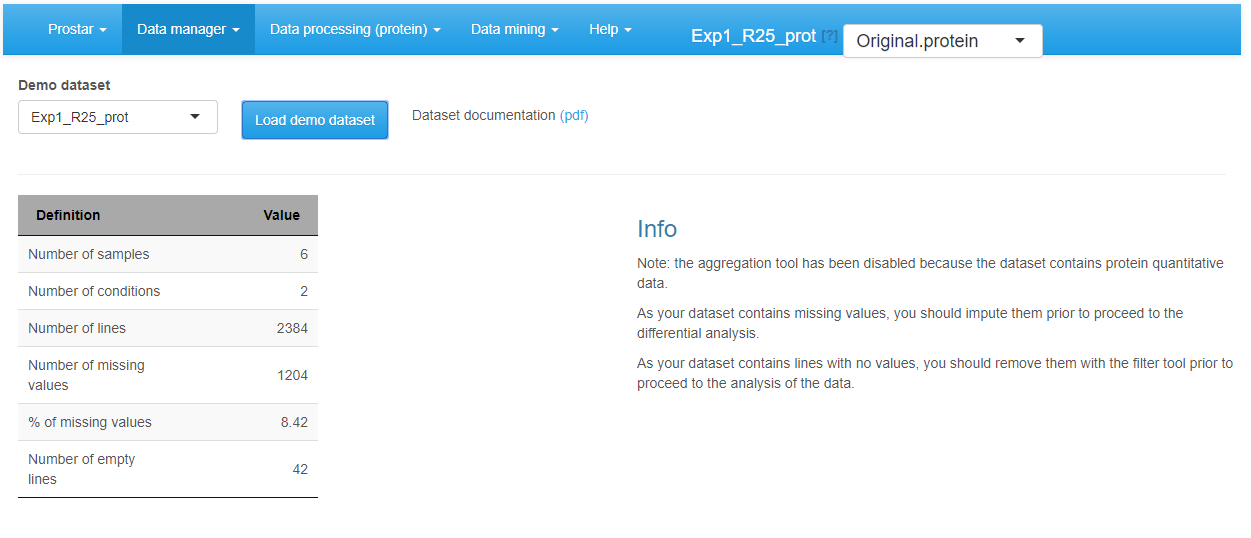
\includegraphics[width=1.00\textwidth]{images/load-prot.png}
\caption{Loading a demo dataset.}
\label{fig:demomodeFig}
\end{figure}

To ease \Biocpkg{Prostar} discovery, a "demo mode" is proposed. In this mode, 
the datasets contained in the package \Biocpkg{DAPARdata} can be directly uploaded to test
\Biocpkg{Prostar} functionalities. To do so, 
simply click on \textbf{Demo data} in the \textbf{Data manager} (Figure~\ref{fig:demomodeFig}).
Note that it possible to display the PDF vignette of the dataset directly from \Biocpkg{Prostar} screen (``Dataset documentation (pdf)'' link).

\subsection{Export} \label{sec:export}
The \textbf{Export} menu from the \textbf{Data manager} gathers all the functionality to save a dataset in various formats, or to compile the results in a scientific report.

\subsubsection{Export a dataset} 
As importing a new dataset from a tabular file is a tedious procedure, we advise to save the dataset as an MSnset binary file right after the conversion (The, it becomes easy to reload it, as detailed in Section~\ref{sec:load}). This makes it possible to restart the statistical analysis from scratch if a problem occurs without having to convert the data another time. Moreover, it is also possible to export the dataset as an Excel spreadsheet (in xlsx format) or as a series of tabulated files grouped in a zipped folder. Any any case, the procedure is similar: 
First, choose the version of the dataset to be saved. Then, choose the desired file format and provide a file name\footnote{Optionally, it is possible to select a subset of the column metadata to make the file smaller.}. Then, click on \textbf{Download} (Figure~\ref{fig:export}). Once the downloading is over, store the file in the appropriate directory.


\begin {figure}
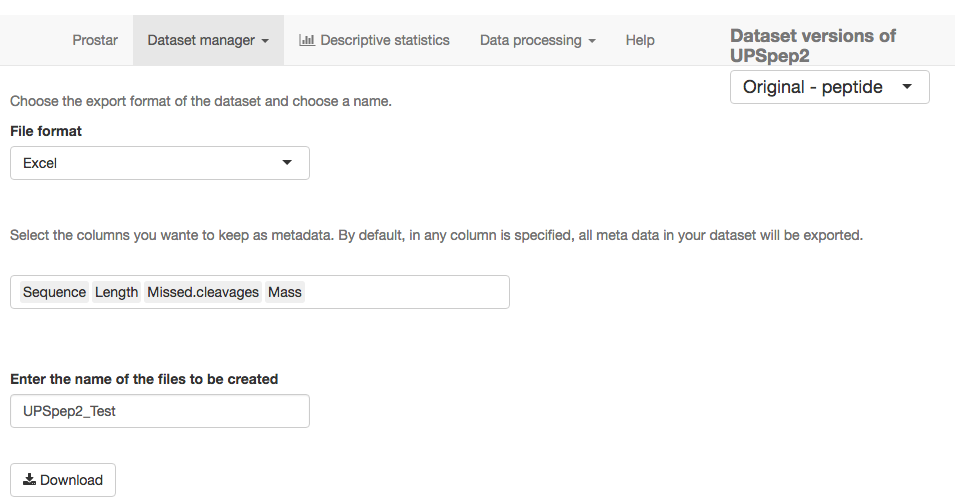
\includegraphics[width=\textwidth]{images/export.png}
\caption{Exporting to an Excel file.}\label{fig:export}
\end {figure}

%%%%%%%%%%%%%%%%%%%%%%%%%%%%%%%%%%%%%%%%%%%%%%%%%
\subsubsection{Build a report (Beta)}\label{sec:Report}

The automatic reporting functionalities are under active development. However, they are still in Beta version and amenable to numerous modifications.
This vignette will be completed with an exhaustive description of \Biocpkg{Prostar} reporting functionality in a near future.

\fixme[TODO]{missing functionality}

%
%\textbf{\textcolor[rgb]{1,0,0}{XXXXXXXXXXXX To be completed XXXXXXXXXXXX}}
%
%
%{The user can download the plots showed in \Biocpkg{Prostar} by 
%right-clicking on the plot. A contextual menu appears and let the user 
%choose either "Save image as" or "Copy image". In the latter case, he/she has 
%to paste the image in appropriate software.}
%
%In addition to the exported datasets (see previous section), the user can generate and download a report, dynamically created on demand (e.g. at the end of an analysis), through the interface presented on Figure~\ref{fig:exportReport}.
%
%The left hand side of the interface shows a list of checkboxes (one for each dataset created during the analysis). By default, all the datasets are selected. The user chooses which results to include in the report. Even if no analysis has been performed (e.g. right after the upload of a dataset), the plots of the Descriptive Statistics panel are available.
%
%The right hand side of the interface allows the user to choose the size and resolution of the images and the format of the report: PDF, HTML or DOC file. 
%
%After selecting the desired options, one clicks on the button "Generate a report". Then, Prostar rebuilds all the required images and includes them in the report file. During this step, the button "Download" remains disabled. Only when the report is ready, the "Download" buttons is enabled.
%
%\begin {figure}
%\centering
%\fbox{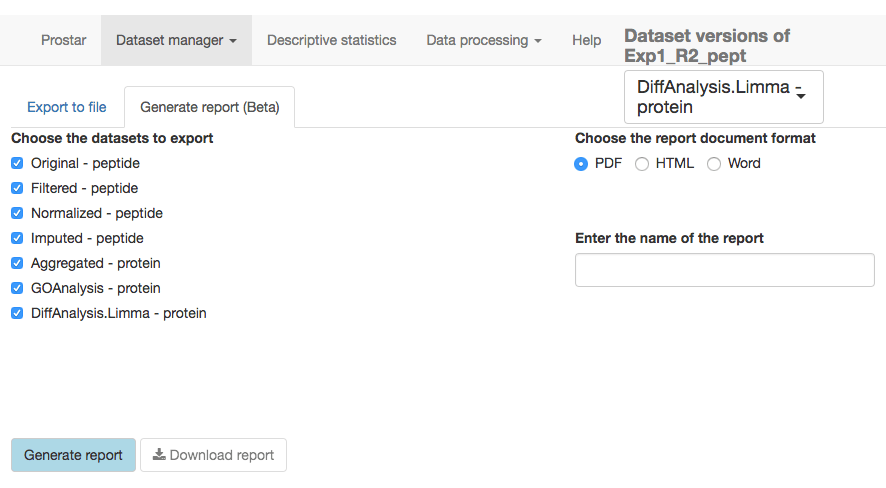
\includegraphics[width=0.9\textwidth]{images/exportReport.png}}
%\caption{Exporting analysis as a report.}\label{fig:exportReport}
%\end {figure}
%
%Please note this report generation functionality is still in Beta version, so that some bugs may remain. In the future, and depending on the users' expectations, the report will be completed: 
%\begin{itemize}
%\item So far, the R commands run for the report generation does not appear in the log console (see \ref{sec:sessionlog});
%\item The texts accompanying the figures is minimal;
%\item The report cannot be customized.
%\end{itemize}
%In the future, we hope to improve it, as well as to generate additional ready-to-use files for  publication (Material \& Methods sketch, R script for reproducibility, etc.)

\section{Data processing}\label{sec:processingadataset}

The \textbf{Data processing} menu contains the 5 predefined steps of a quantitative 
analysis. They are designed to be used in a specific order:
\begin{enumerate}
\item {Filtering}
\item{Normalization}
\item{Imputation}
\item{Aggregation} (only for peptide-level data)
\item{Hypothesis testing}
\end{enumerate}
For each step, several algorithms or parameters are available, all of them being 
thoroughly detailed in the sequel of this section.

During each of these steps, it is possible to test several options, and to 
observe the influence of the processing in the descriptive statistics menu 
(see Section~\ref{sec:descriptivestatistics}), which is dynamically updated. 

Finally, once the ultimate tuning is chosen for a given step, it is advised 
to save the processing. By doing so, another dataset appears in the Dataset 
versions list (see Section~\ref{sec:availabledatasets}). Thus, it is possible 
to go back to any previous step of the analysis if necessary, without starting 
back the analysis from scratch.

%%%%%%%%%%%%%%%%%%%%%%%%%%%%
\subsection{Filtering}\label{sec:filtering}
In this step, the user may decide to delete several peptides or proteins 
according to two criteria: First is the amount of missing values (if it is
too important to expect confident processing, see tab 1); 
Second is string-based filtering (some analyte can be deleted after having been
tagged, such as for instance reverse sequences in target-decoy approaches, or
known contaminants, see tab 2).

\begin {figure}
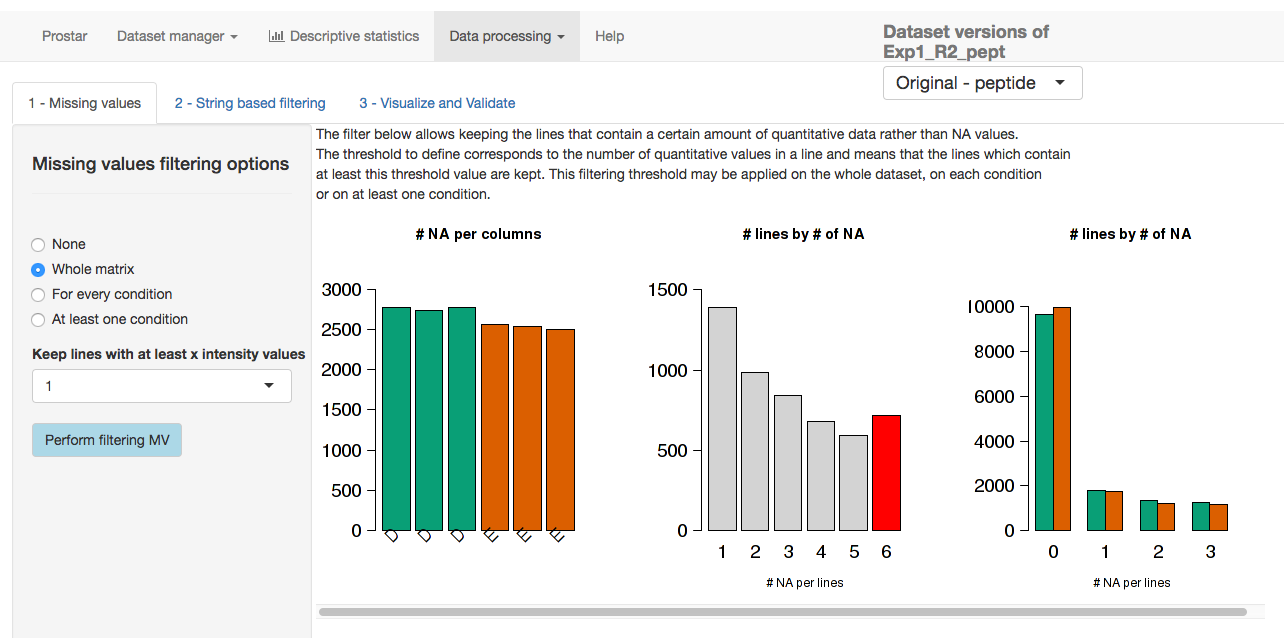
\includegraphics[width=\textwidth]{images/filter1.png}
\caption{Interface of the filtering tool - 1.}\label{fig:filter1}
\end {figure}

To filter the missing values (first tab called \textbf{Missing values}), the choice 
of the lines to be deleted is made by different options (see 
Figure~\ref{fig:filter1}):
\begin {itemize}
\item\textbf{None}: No filtering, the quantitative data is left unchanged. 
This is the default option;
\item\textbf{Empty lines}: Only the lines with 100\% of missing values 
(analytes that have been identified but not quantified) are filtered out.
\item\textbf{Whole Matrix}: The lines (across all conditions) in the 
quantitative dataset which contain less non-missing value than a 
user-defined threshold are deleted;
\item\textbf{For every condition}: The lines for which each condition 
contain less non-missing value than a user-defined threshold are deleted;
\item\textbf{At least one condition}: The lines for which at least one 
condition contain less non-missing value than a user-defined threshold 
are deleted;
\end {itemize}

To visualize the effect of the filtering options (without saving the changes or
impacting the current dataset), just click on \textbf{Perform filtering}. 
If the filtering does not 
produce the expected effect, it is possible to test another one. To do so, one 
simply has to choose another method in the list and click again on \textbf{Perform 
filtering}. The plots are automatically updated. This action does not modify 
the dataset but offers a preview of the filtered data. The user can visualize 
as many times he/she wants several filtering options.

\begin {figure}
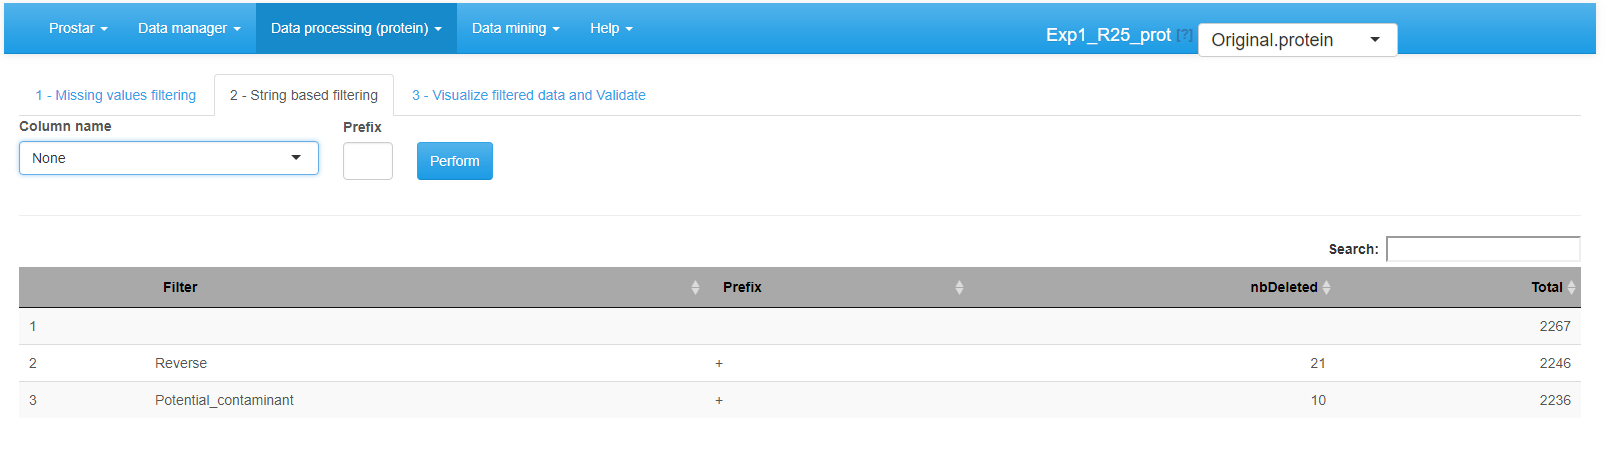
\includegraphics[width=\textwidth]{images/filter2.png}
\caption{Interface of the filtering tool - 2.}\label{fig:filter2}
\end {figure}

Afterward, proceed to the \textbf{String based filtering},
where it is possible to filter out proteins according to information stored in the metadata.
To do so: Among the columns constituting the protein metadata listed in the drop-down menu, 
select the one containing the information\footnote{To work properly, the selected column must 
contain information encoded as a string of characters. For each protein, the beginning of 
the corresponding string is compared to a given prefix. If the prefix matches, the protein is filtered out. 
Otherwise, it is conserved in the protein list. Note that the filter only operates a prefix search 
(at the beginning of the string), not a general tag match search (anywhere in the string). 
Similarly, filters based on regular expressions are not implemented.}
of interest (for instance, 
``Contaminant'' or ``Reverse'')\footnote{In datasets resulting from a MaxQuant, 
metadata indicates under a binary form which proteins are reversed sequences 
(resulting from a target-decoy approach) and which are potential contaminants. 
Both of them are indicated by a ``+'' in the corresponding column (the other 
proteins having an NA instead). It is thus possible to filter both reversed and 
contaminants out by indicating ``+'' as the prefix filter. However, if adequately encoded, 
filtering on other type of information is possible.}. Then, specify in each case 
the prefix chain of characters that identifies the proteins to filter\footnote{If one 
has no idea of the prefixes, it is possible to switch to the \textbf{Data Explorer} 
in the \textbf{Descriptive Statistics} menu (see Section~\ref{sec:descriptivestatistics}), 
so as to visualize the corresponding metadata.}.
Click on \textbf{Perform} to remove the corresponding proteins. 
A new line appears in the table listing all the filters that have been applied.
If other string-based filters must be applied, iterate the same process as many times
as necessary.

\begin {figure}
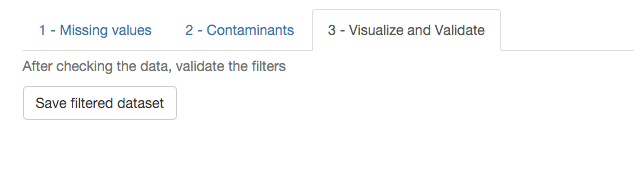
\includegraphics[width=\textwidth]{images/filter3.png}
\caption{Interface of the filtering tool - 3.}\label{fig:filter3}
\end {figure}

Once the filtering is appropriately tuned,go to the last tab 
(called \textbf{Visualize filtered data and validate}) (see Figure~\ref{fig:filter3}), to visualize 
the set of analytes that have been filtered.  
Finally, click on \textbf{Save filtered dataset}. 
A new dataset is created; it becomes the new 
current dataset and its name appears in the dropdown menu upper right corner 
of the screen. All plots and tables available in \Biocpkg{Prostar} 
are automatically updated.

%%%%%%%%%%%%%%%%%%%%%%%%%%%%
\subsection{Normalization}\label{sec:normalization}

The next processing step proposed by Prostar is data normalization. 
Its objective is to reduce the biases introduced at any preliminary 
stage (such as for instance batch effects).
\Biocpkg{Prostar} offers a number of different normalization 
routines that are described below.

To visualize the influence of the normalization, three plots are displayed
(see Figure~\ref{fig:norma}):
The first two plots are those of the \textbf{Intensity distribution} tab of the 
\textbf{Descriptive statistics} (see Section~\ref{sec:densityplot}).
The last one depicts the distortion induced by the chosen normalization 
method on each sample.

\begin {figure}
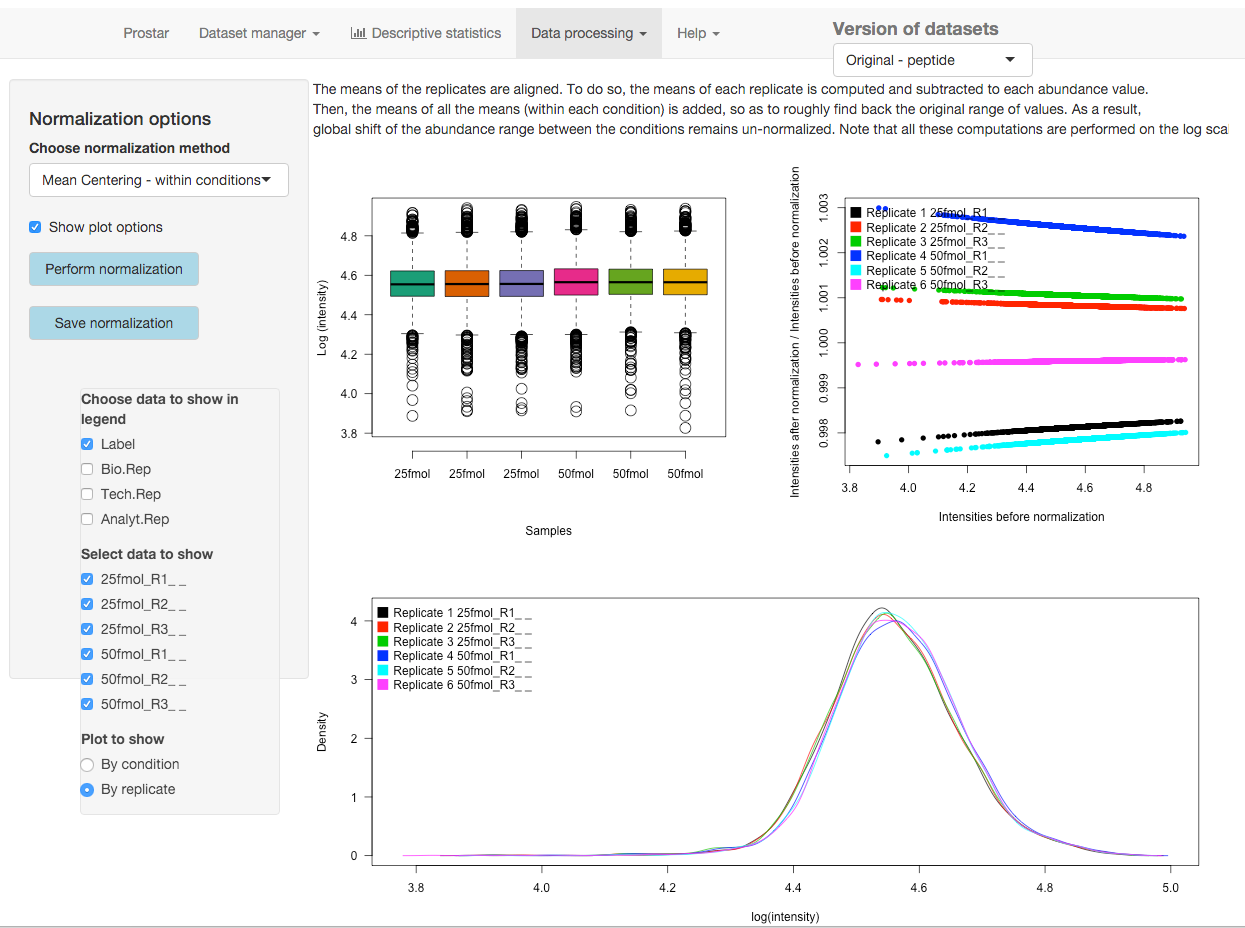
\includegraphics[width=\textwidth]{images/normalisation.png}
\caption{Interface of the normalization tool.}\label{fig:norma}
\end {figure}

Choose the normalization method among the following ones:
\begin{enumerate}
	\item \textbf{None}: No normalization is applied. This can be useful in case of tightly calibrated proteomics experiments (such as spiked-in or benchmark samples), where normalization may be more harmful than useful. Moreover, when testing several normalizations, clicking on ``None'' is useful to recover the original distribution, which serves as reference to compare the methods.
	\item \textbf{Global quantile alignment}: The Quantile of the intensity distributions of all the samples are equated, as proposed by the \Rfunction{normalize.quantiles()} of \Biocpkg{preprocessCore}. This method proposes a normalization of important
magnitude that should be cautiously used. It practically amounts to replace 
abundances by order statistics. 
	\item \textbf{Column sums}: The total intensity values of all the samples are equated. The rationale behind is to normalize according to the total amount of biological material within each sample. Thus, this normalization is interesting to compare the proportions of a given 
     protein in different samples that do not necessarily contain the same 
     amount of biological material. Contrarily to the others, this 
     normalization is not performed on the log2 scale, for it would not have 
     any interpretation (the data are thus exponentiated and 
     re-log2-transformed as pre-and post-processing)
	
	\item \textbf{Quantile Centering}: A given quantile of the intensity distribution is used as reference\footnote{This normalization method should not be confused with Global quantile alignment.}. 
It proposes to shift the sample distributions 
(either all of them at once, or within each condition at a time) to align a specific 
quantile: the median (under the assumption that up-regulations and down-regulations 
are equally frequent), the 15\% quantile (under the assumption that the signal/noise ratio is 
roughly the same in all the samples), or any other user's choice.
	\item \textbf{Mean Centering}: sample intensity distributions are aligned on their mean intensity values (and optionally, the variance distributions are equated to one).
	\item \textbf{VSN}: (or Variance Stabilizing Normalization) from the \Biocpkg{vsn} package. Its objective is to have the analyte variance independent of the intensity. Note that this normalization is computed on the original intensity values, not the log2 transformed ones. The result from the normalization is not in the log2 scale, nor in the original one, but in-betwee: the scale is roughly linear for low-intensity values and roughly logarithmic for high-intensity values (so as to avoid the logarithm singularity).
	\item \textbf{LOESS normalization}: The intensity values are normalized by means of a local regression model of the difference of intensities as function of the mean intensity value, as implemented in the \Rfunction{normalizeCyclicLoess()} from \Biocpkg{limma} package.
\end{enumerate}

Then, for each normalization method, the interface is automatically updated to display the method parameters that must be tuned. Notably, for most of the methods, it is necessary to indicate whether the method should apply to the entire dataset at once (the \textbf{overall} tuning), or whether each condition should be normalized independently of the others (the \textbf{within conditions} tuning). 

Other parameters are method specific:
\begin{itemize}
	\item \textbf{Quantile centering}: It is necessary to define the quantile of the intensity distribution that is used as reference. The most classically used is the median (quantile 0.5), but other quantiles can aslo be useful, depending on the dataset. Notably, as the lower limit of quantitation is roughly constant over the samples, relying on a lower quantile such as 0.15 can be efficient to alilgn the signal/noise ratios.
	\item \textbf{Mean centering}: It is necessary to indicate whether the distribution variances are scaled to 1.
	\item \textbf{LOESS}: The span corresponds to the proportion of the other analytes that are considered to perform the regression.
\end{itemize}

Once the method is correctly parametrized, click on \textbf{Perform normalization}.
Observe the influence of the normalization method on the graphs. %Optionally, click on "Show plot options", so as to tune the graphics for a better visualization.
If the result of the normalization does not correspond to the expectations, change the normalization method or change its tuning.
Once the normalization is effective, click on \textbf{Save normalization}.
Check that a new version appears in the dataset version drop-down menu, referred to as \textbf{Normalized - Protein} or \textbf{Normalized - Peptide}.

\subsection{Imputation}\label{sec:imputation}
\subsubsection{Focus on: Missing value nomenclature}\label{sec:vmnomenclature}
Classically, missing values are categorized according to their underlying missingness mechanism:
\begin{itemize}
	\item \textbf{Missing Completely At Random (MCAR)}: This category of missing values gather
	all those which result from the combination and propagation of multiple minor errors or 
	stochastic fluctuations. As a result, each missing value cannot be directly explained 
	by the nature of the analyte, nor by its measured intensity. MCAR values are assumed to 
	distribute uniformely in the dataset as well as along the intensity range. 
	\item \textbf{Missing Not At Random (MNAR)}: On the contrary, MNAR have a more precise cause.
	Notably, in mass spectrometry-based analysis, chemical species whose abundance are too close 
	to the lower limit of detection of the instrument record a higher rate of missing values. This is why,
MNAR-devoted imputation methods used in proteomics focus on left-censored data (that
is, the distribution of which with respect to the abundance is truncated on the left side,
i.e. on the region depicting the lower abundances).
\end{itemize}

However, it also makes sense to classify the missing value according to the analyte they impact, regardless of
the underlying mechanism. This is why, in \Biocpkg{Prostar}, it has been decided to separate:
\begin{itemize}
	\item \textbf{POV} (standing for \textbf{Partially Observed Value}).
	\item \textbf{MEC} (standing for \textbf{Missing in the Entire Condition}).
\end{itemize}
All the missing values for a given protein in a given condition are considered POVs \textbf{if and only if there is at least one observed value for this protein in this condition}. Alternatively, \textbf{if all the intensity values are missing for this protein in this condition}, the missing values are considered MECs.
As a result, each missing values is either POV or MEC. Moreover, for a given protein across several conditions, the missing values can split into POVs and MECs, even though within a same condition they are all of the same type.

With the default color setting, POVs are depicted in light blue and MECs in light orange.

In \Biocpkg{Prostar}, the following assumptions are made:
\begin{itemize}
	\item \textbf{In peptide-level datasets}, it is either possible to consider all the missing values, either POVs or MECS, as of the same type and to blindly apply one of the \textbf{basic methods} proposed. As a more refined alternative, we propose to rely on \Biocpkg{imp4p}, which considers that:
	\begin{itemize}
		\item MECs should always assumed to be MNAR. Note that imputing MEC values is a real issue as, in the condition of interest, there is no observed value to rely the imputation on.
		\item No assumption should be made on POVs: they can be a mix of MCAR and MNAR values, and the missingness mechanism of each is diagnosed before the imputation, thanks to an \Biocpkg{imp4p} routine.
	\end{itemize}
		\item \textbf{In protein-level datasets}:
	\begin{itemize}
		\item The number of POVs is generally not large enough to perform an accurate diagnosis of the POV missingness mechanism, as proposed with \Biocpkg{imp4p} at peptide-level. Thus, they are all assumed to be MCAR. 
		\item MECs are always assumed to be MNAR and imputed accordingly. 
	\end{itemize}
\end{itemize}
As a whole, it is advised to work at peptide-level rather than protein-level, and to use the refined imputation mechanism of \Biocpkg{imp4p}.

\textbf{Remarks}: 
\begin{itemize}
	\item Sometimes, an analyte (and not a missing value) can be referred to as \textbf{Lapala}, when it has both observed values and MEC (which means it is observed in some conditions and not observed in others). This term was coined from French "l\`a/pas-l\`a"(meaning "here/not-here").
	\item Contrarily to the normalization step, where it is possible to choose between \textbf{within conditions} and \textbf{overall} application of the algorithm, the imputation step cannot be applied overall-wise, but only condition-wise. The rationale behind is that in case of very different conditions, it does not make sense to rely on the observed values of one condition to impute those of the others. With this regards, \Biocpkg{Prostar} strongly differs from most of the other proteomics software tools, where the imputation can borrow information from multiple independent conditions.
\end{itemize}
 
\subsubsection{Protein-level imputation}\label{sec:proteinimputation}
As a consequence of the previous paragraph, in protein-level datasets, \Biocpkg{Prostar} proposes to use an MCAR-devoted imputation algorithm for POVs, and an MNAR-devoted one for MECs.

\begin {figure}
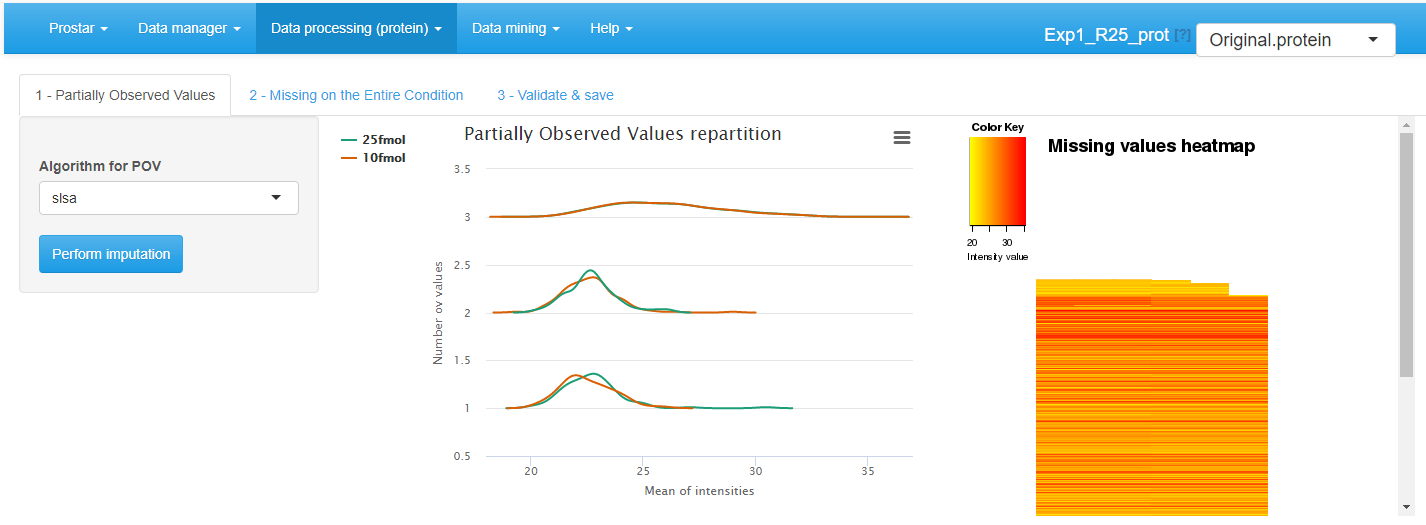
\includegraphics[width=\textwidth]{images/protein-POV.png}
\caption{POV imputation}\label{fig:prot-POV}
\end {figure}

On the first tab (see Figure~\ref{fig:prot-POV}), select the algorithm to impute POV values, among the following ones, and tune its parameter accordingly:
\begin{itemize}
	\item \textbf{None}: No imputation is performed for POVs.
	\item \textbf{SLSA} (Structured Least Square Adaptative): It is a regression based imputation method which account for a possible hierachical design. It does not require any parameter tuning.
	\item \textbf{DetQuantile}: It is advised to use DetQuantile to impute MECs rather than POVs, however, in some case, it may be interesting to rely on a single imputation method for all the missing values. This is why, this method is proposed also proposed for POV imputation. DetQuantile description and parameter tuning is described below.
	\item \textbf{KNN} (K-nearest neighbors):  KNN imputation proposes to estimate each missing value by the mean of the observed values of other proteins with a similar intensity pattern (called neighbors). One only has to tune $K$, the number of neighbors to account for. The method simply wraps the one of the \Biocpkg{impute} package, however, contrarily to the classical implementation and use, the function processes one condition at a time, rather than all the conditions at once. 
\end{itemize}
According to our expertise, we advise to select the \textbf{SLSA} algorithm from \CRANpkg{imp4p} but the other methods can also be of interest in specific situations.

The first distribution plot depicts the mean intensity of each condition conditionally to the number of missing values it contains.
It is useful to check that more values are missing in the lower intensity range (due to left censorship).

The heatmap on the right hand side clusters the proteins according to their 
distribution of missing values across the conditions. Each line of the map 
depicts a protein. On the contrary, the columns do not depicts the replicates 
anymore, as the abundance values have been reordered so as to cluster the 
missing values together. Similarly, the proteins have been reordered, so as 
to cluster the proteins that have a similar amount of missing values 
distributed in the same way over the conditions. Each line is colored so as 
to depicts the mean abundance value within each condition. This heatmap is 
also helpful to decide what is the main origin of missing values (MCAR or MNAR).

Click on \textbf{Perform Imputation}. A short text shows up to summarize the result of the imputation, but the graphics are not updated.
However, the next tab is enabled, on which the plots are updated with the imputation results.

After POVs, it is possible to deal with MECs. As a matter of fact, it is always dangerous to impute them, as in absence of any value to rely on, the imputation is arbitrary and risks to spoil the dataset with maladjusted values. As an alternative, it is possible to (1) keep the MEC as is in the dataset, yet, it may possibly impede further processing, (2) discard them at the filter step (see Section~\ref{sec:filtering}) so as to process them separately. However, this will make it impossible to include these proteins (and their processing) in the final statistics, such as for instance FDR. 

For MEC imputation, several methods are available (see Figure~\ref{fig:prot-MEC}):
\begin{itemize}
	\item \textbf{None}: If MEC are not going to be imputed, this is what to select.
	\item \textbf{DetQuantile}: It proposes to impute each missing value within a given sample by a deterministic value (usually a low value). The rationale behind is that MEC values corresponds to proteins that are below the quantification limit in one condition, so that they should not be imputed according to observed values in the other conditions. Although the use of a deterministic value slightly disturb the intensity distribution, it makes the MEC values easy to spot, as they all correspond to a known numerical value. Concretely, the imputation value is chosen as a (small) \textbf{quantile} -the first parameter) of each sample distribution. Depending on the dataset, a quantile between 1\% and 5\% should be used, depending on the stringency you want to apply on proteins quantified only in one condition of a pairwise comparison. In case of a dataset with too few proteins, the lower quantile may lead to instable values. In such a case, we advise to use a larger quantile value (for instance 10\% or greater) but to use a smaller multiplying \textbf{factor} (the second parameter) so as to keep the imputation value reasonably small with respect to the detection limit (for instance, consider a factor of 0.2 or smaller). In any case, when using detQuantile, the list of imputation values for each sample appears above the graphics.
	\item \textbf{Fixed value}: As an alternative, it is possible for the user to tune the imputation with a specific value that will be used in all samples of all conditions. Although appealing for its simplicity, this method may lead to important data distortion, so it is advised to use \textbf{detQuantile} algorithm whenever possible.
\end{itemize}
Based on our experience, we advise to use \textbf{detQuantile} algorithm.

Click on \textbf{Perform Imputation}. A short text shows up to summarize the result of the imputation, but the graphics are not updated.
As the imputation is finished, the updated plots would not be informative, so they are not displayed on the final tab (referred to as \textbf{Validate \& save}).
Note that when displaying or exporting the data, the color code used with missing values is still used for the imputed values, so that at any moment, it is possible to trace which proteins were imputed.

\begin {figure}
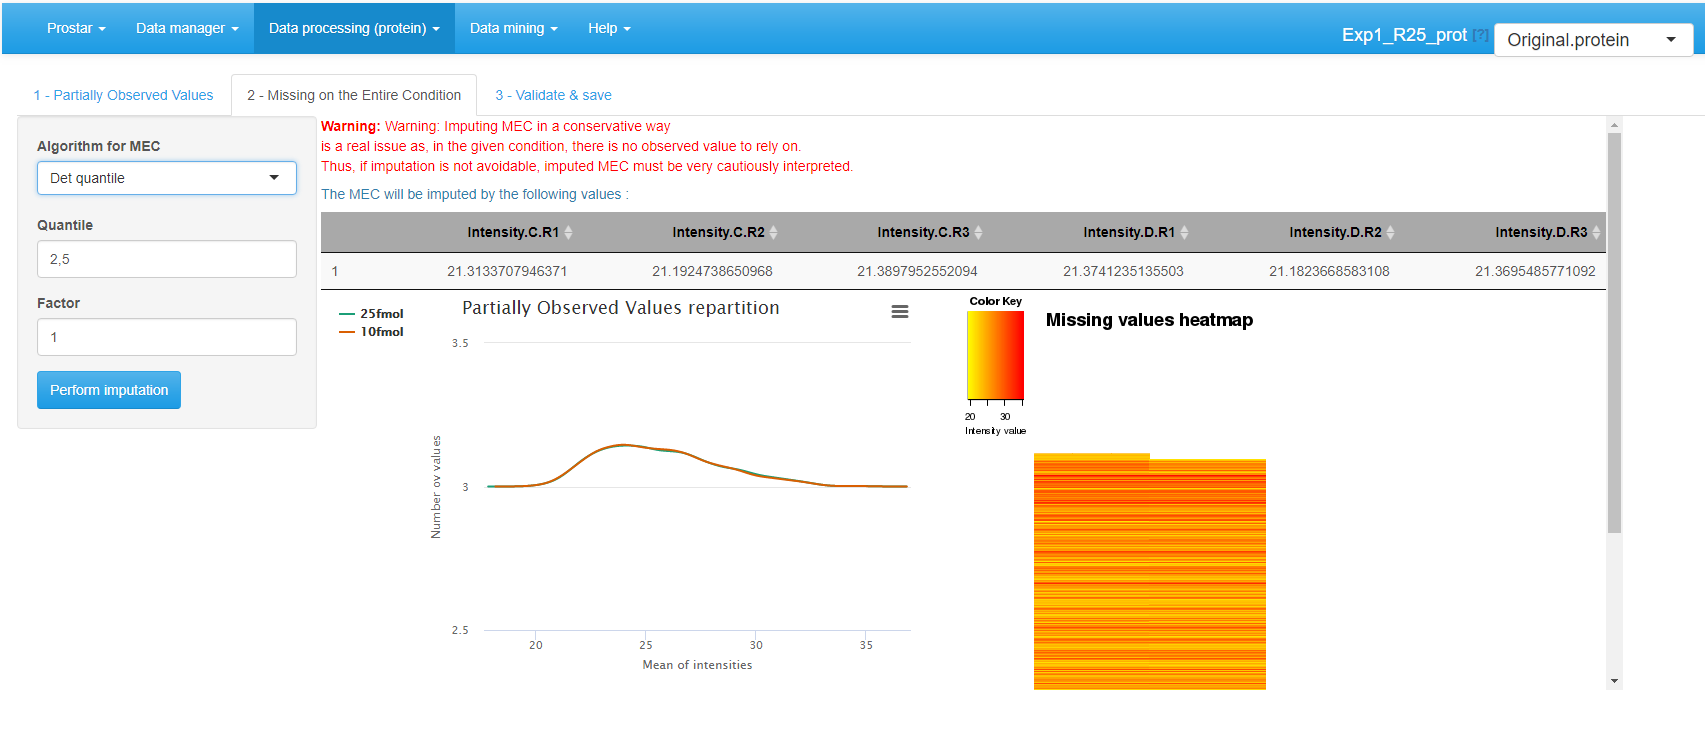
\includegraphics[width=\textwidth]{images/protein-MEC.png}
\caption{POV imputation}\label{fig:prot-MEC}
\end {figure}

\subsubsection{Peptide-level imputation}\label{sec:peptideimputation}

Notice that at peptide level, many lines of the dataset may corresponds to identified peptides with no quantification values.
In order to avoid spoiling the dataset with their meaningless imputed values, it is demanded to filter them before proceeding (see Section~\ref{sec:filtering}). 

Two plots are available in order to facilitate the understanding of the missing value distribution.
These plots are the same as for protein-level imputation:

The distribution plot on the left depicts the mean intensity of each condition 
conditionally to the number of missing values it contains.
It is useful to check that more values are missing in the lower intensity 
range (due to left censorship).

The heatmap on the right hand side clusters the proteins according to their 
distribution of missing values across the conditions. Each line of the map 
depicts a protein. On the contrary, the columns do not depicts the replicates 
anymore, as the abundance values have been reordered so as to cluster the 
missing values together. Similarly, the proteins have been reordered, so as 
to cluster the proteins that have a similar amount of missing values 
distributed in the same way over the conditions. Each line is colored so as 
to depicts the mean abundance value within each condition. This heatmap is 
also helpful to decide what is the main origin of missing values (MCAR or MNAR).

\begin {figure}
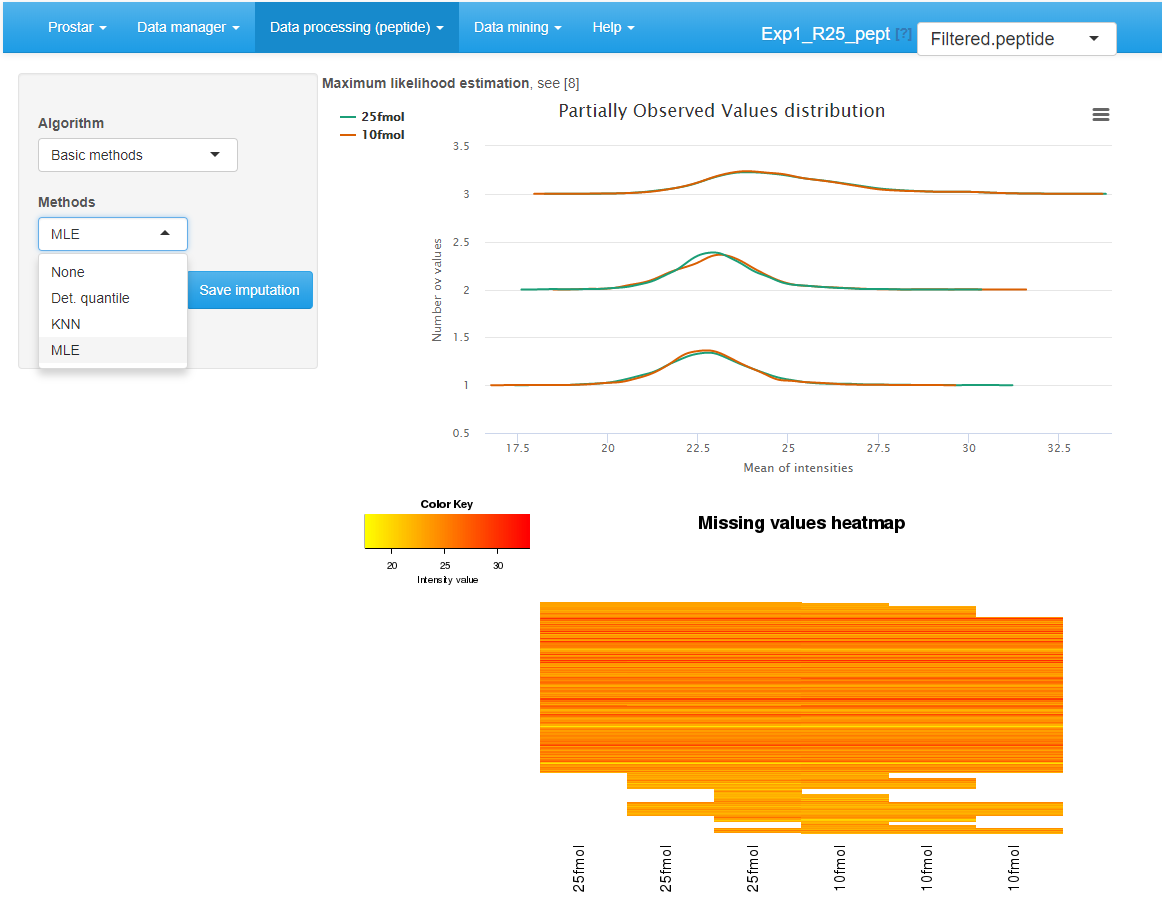
\includegraphics[width=\textwidth]{images/peptide-basicImputation.png}
\caption{Interface of the imputation of missing values tool.}\label{fig:peptide-bimp}
\end {figure}

To impute the missing peptide intensity values, it is either possible to rely on
classical methods of the state of the art, or to use \CRANpkg{imp4p}. The former
ones are available by choosing \textbf{Basic methods} in the \textbf{Algorithm} 
drop-down menu (see Figure~\ref{fig:peptide-bimp}). Another drop-down menu appears proposing one of the following methods:
\begin{itemize}
	\item \textbf{None}: No imputation is performed. This option is convenient to recover the original missing value distribution when comparing several imputation methods.
	\item \textbf{DetQuantile}: It proposes to impute each missing value within a given sample by a deterministic value (usually a low value). The rationale behind is that MEC values corresponds to peptides that are below the quantification limit in one condition, so that they should not be imputed according to observed values in the other conditions. Although the use of a deterministic value slightly disturb the intensity distribution, it makes the MEC values easy to spot, as they all correspond to a known numerical value. Concretely, the imputation value is chosen as a (small) \textbf{quantile} -the first parameter) of each sample distribution. Depending on the dataset, a quantile between 1\% and 5\% should be used, depending on the stringency you want to apply on proteins quantified only in one condition of a pairwise comparison. In case of a dataset with too few analytes (which is more likely to be the case at protein-level than at peptide-level), the lower quantile may lead to instable values. In such a case, we advise to use a larger quantile value (for instance 10\% or greater) but to use a smaller multiplying \textbf{factor} (the second parameter) so as to keep the imputation value reasonably small with respect to the detection limit (for instance, consider a factor of 0.2 or smaller). In any case, when using detQuantile, the list of imputation values for each sample appears above the graphics.
	\item \textbf{KNN} (K-nearest neighbors):  KNN imputation proposes to estimate each missing value by the mean of the observed values of other peptides with a similar intensity pattern (called neighbors). One only has to tune $K$, the number of neighbors to account for. The method simply wraps the one of the \Biocpkg{impute} package, however, contrarily to the classical implementation and use, the function processes one condition at a time, rather than all the conditions at once. 
	\item \textbf{MLE} (Maximum Likelihood Estimation): This method, from the \Biocpkg{norm} package, propose to estimate the expected abundance value of each peptide in each condition (with the maximum likelihood estimate), and to use this expected value as replacement of missing values. There is no parameter to tune with MLE imputation.
\end{itemize}

All these methods are applied on all missing values, without diagnosing their nature, as explained in Section~\ref{sec:vmnomenclature}.
Alternatively, it is possible to rely on \CRANpkg{imp4p} (see Figure~\ref{fig:peptide-imp4p}). It works as follows:
\begin{enumerate}
	\item For POVs, a diagnosis of the nature of each missing value is perform. As an output each POV is endowed with a probability of being either MNAR or MCAR.
	\item Several iterations (as many as tuned on the interface, default is 10 - the more iteration, the more accurate the imputation) of the following algorithm are performed:
		\begin{itemize}
			\item Randomly assign each POV to either MCAR or MNAR, according to its diagnosis probability.
			\item If it is MCAR, SLSA algorithm is used for imputation.
			\item If it is MNAR, IGCDA algorithm is used for imputation.
		\end{itemize}
	\item All the POV imputed values computed along the iterations are average to provide the imputation final results.
	\item Optionally, it is possible to impute the MECs. To do so, one relies on a slightly modified version of IGCDA, which requires tuning 2 parameters: First is the upper bound of the MNAR imputed values, expressed as a quantile of the distribution of observed values in each sample (default is centile 2.5). Second is the probability distribution defined on the trange of MNAR values (either uniform or beta): Beta is more conservative, as it provides more weight on values that are close to the detection limit, which reduces the risk of creating artificial differentially abundant peptides (and thus proteins).
\end{enumerate}

\begin {figure}
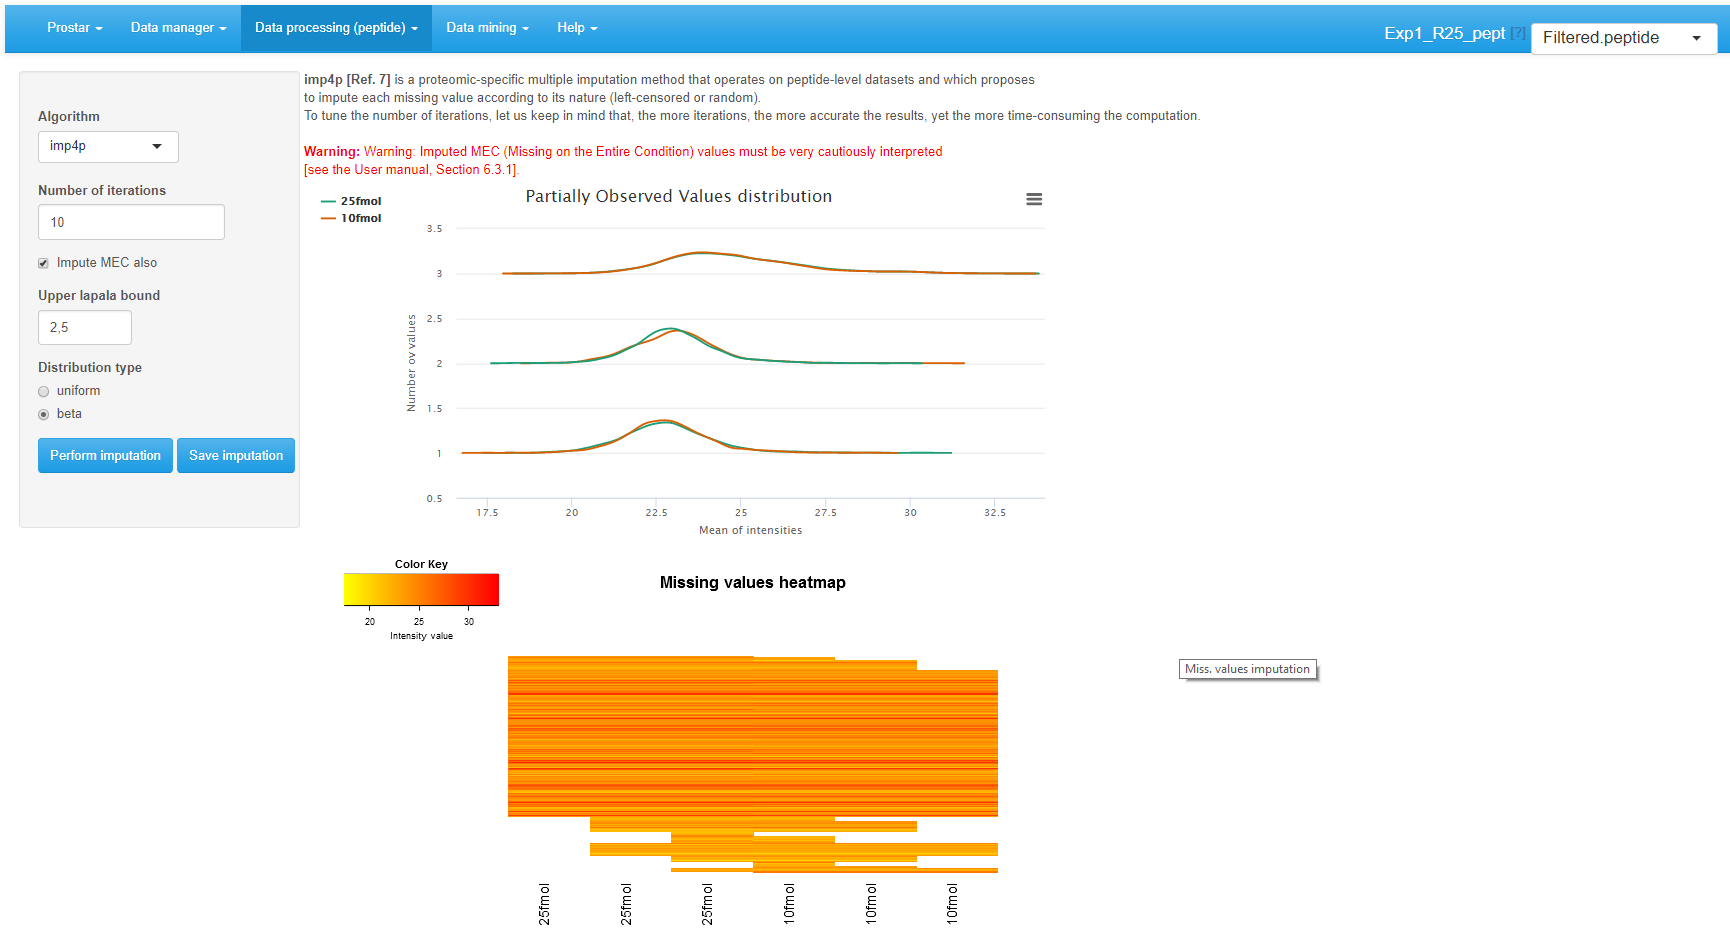
\includegraphics[width=\textwidth]{images/peptide-imp4p.png}
\caption{Interface of the imputation of missing values tool.}\label{fig:peptide-imp4p}
\end {figure}

It is possible to directly visualize the effect of an imputation method on the updated plots. 
If the imputation does not produce the expected effect, 
it is possible to test another one. To do so, one chooses another 
method in the list and click on \textbf{Perform imputation}. 
This action does not modify the dataset but offers a 
preview of the imputed quantitative data.
It is possible to visualize as many imputation methods/tuning as desired. 
Once the correct one is found, one validates the choice by clicking on 
\textbf{Save imputation}. Then, a new "imputed" dataset is created and loaded in 
memory. This new dataset becomes the new current dataset and the "Imputed" version
appears in the upper right drop-down menu. All plots and 
tables in other menus are automatically updated.

%%%%%%%%%%%%%%%%%%%%%%%%%%%%%%
\subsection{Aggregation}\label{aggregation}

This steps only hold for peptide-level dataset. Its purpose is to build a 
protein-level dataset on the basis of the peptide intensities that have been
processed in \Biocpkg{Prostar}.

If this step has not been fulfilled at the initial data conversion (see Section~\ref{sec:import}),
it is first necessary to specify which column metadata of the peptide-level dataset
contains the parent protein IDs (which will be used to index the protein-level
dataset that is going to be created).

 
Once the parent protein IDs are specified, two barplots are displayed 
(see Figure~\ref{fig:aggregation}). They provide the distribution 
of proteins according to their number of peptides (either all of them, or 
only those which are specific to a single protein). These statistics are 
helpful to understand the distribution of shared peptides, as well as the
peptide/protein relationships.

\begin {figure}
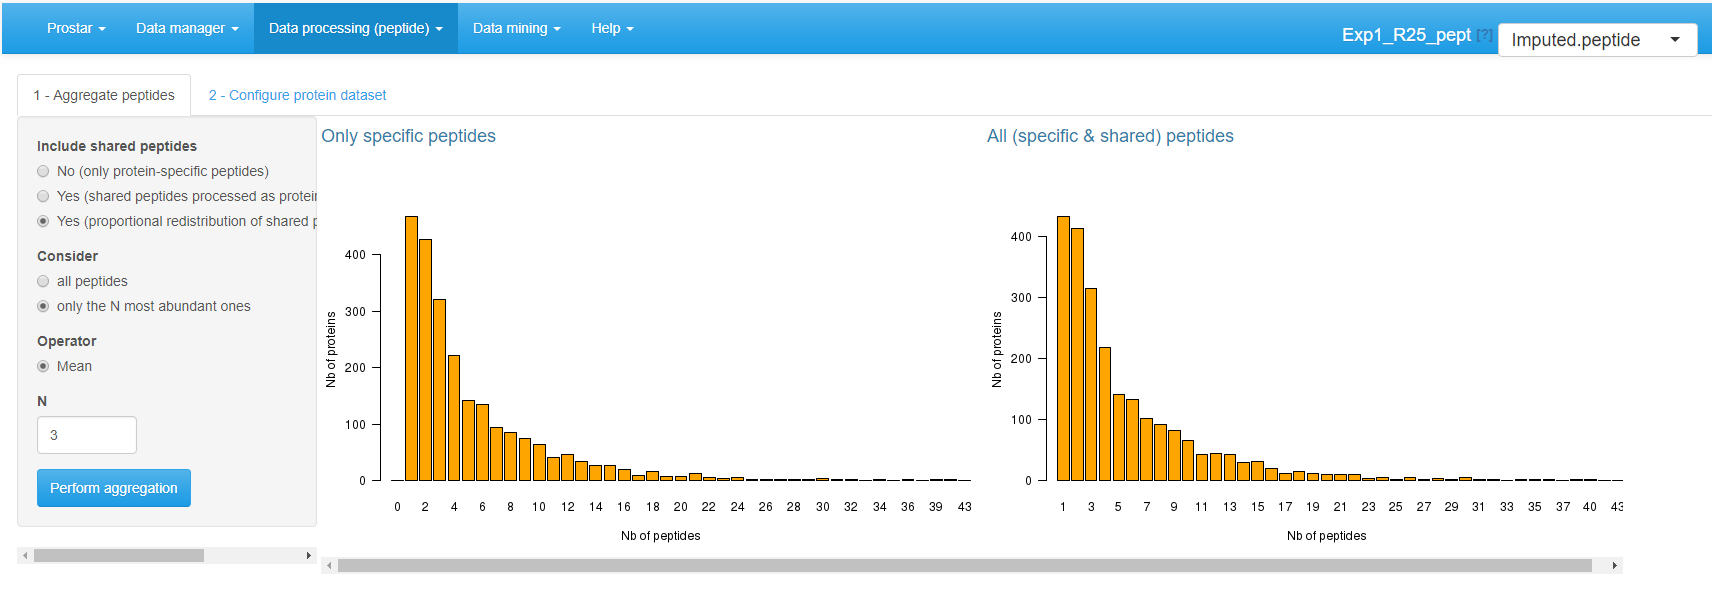
\includegraphics[width=\textwidth]{images/aggregation.png}
\caption{Aggregation screen}\label{fig:aggregation}
\end {figure}

Aggregation requires to tune the following parameters:
\begin{itemize}
	\item \textbf{Include shared peptides}: Here, one defines if protein intensity should be defined only by aggregating protein-specific peptides, or if (and thus how) shared peptides should be included. If shared peptides are not included, one faces the risk of losing some proteins (those which do not have a single specific peptide). Three options are available:
	\begin{itemize}
		\item \textbf{No (only protein-specific peptides)}.
		\item \textbf{Yes (shared peptides processed as protein specific)}.
		\item \textbf{Yes (proportional redistribution of shared peptides)}. This last option is the most accurate one, yet, it is slower, for proportional redistribution is iterated as many time as necessary to reach convergence.
	\end{itemize}
	\item \textbf{Consider}: The user specifies which peptides should be considered for aggregation.
	\begin{itemize}
		\item \textbf{All peptides}, regardless of their intensities.
		\item \textbf{Only the $N$ most abundant ones}. In such a case, one has to specify a value for $N$.
	\end{itemize}
	\item Finally, one defines the aggregation \textbf{Operator}: Sum or Mean. However, in case of proportional redistribution of the shared peptide intensities, only the mean operator is available.
\end{itemize}
 
Once the aggregation is appropriately tuned, click on \textbf{Perform aggregation}.

On the second tab, one selects the columns of the peptide dataset that 
should be kept in the metadata of the protein dataset (e.g. the 
sequence of the peptides). For any 
given parent-protein, the corresponding information of all of its child-peptides  
will be grouped and stored in the protein dataset metadata. Once done, one clicks 
on \textbf{Save aggregation}. This creates a new "aggregated" dataset that
is directly loaded in memory. 

As the new dataset is a protein one, the \textbf{Aggregation} menu has been disabled. 
Thus, the interface automatically switches to the homepage. However, the aggregated 
dataset is accessible and can be analyzed (in the \textbf{Data mining} menu) and processed (in
the \textbf{Data processing} menu).

The aggregation being more computationaly demanding than other processing 
steps, the current version of \Biocpkg{Prostar} does not provide the same 
flexibility regarding the parameter tuning. Here, it is necessary to save the 
aggregation result first, then, check the results in the \textbf{Descriptive statistics},
and possibly to go back to the imputed dataset with the dataset 
versions dropdown menu to test another aggregation tuning. Contrarily to 
other processing steps, it is not possible to visualize on-the-fly the 
consequences of the parameter tuning, and to save it afterward. 

Naturally, the output of this step is not a peptide dataset anymore, but a 
protein dataset. As a result, all the plots available in \Biocpkg{Prostar} 
are deeply modified. Notably, all those which are meaningless at a protein-level
are not displayed anymore.


%%%%%%%%%%%%%%%%%%%%%%%%%%%%%%%%%%%%%%%%%%%%%%%%%%%%%%%%
\subsection{Hypothesis testing}\label{sec:hp}

\subsubsection{Peptide-level}\label{sec:peptidehp}

\fixme[TODO]{missing functionality}

\subsubsection{Protein-level}\label{sec:proteinhp}
For datasets that do not contain any missing values, 
or for those where these missing values have been imputed, 
it is possible to test whether each protein is significantly 
differentially abundant between the conditions.
To do so, click on \textbf{Hypothesis testing} in the \textbf{Data processing} menu (see Figure~\ref{fig:hp}). 

\begin {figure}
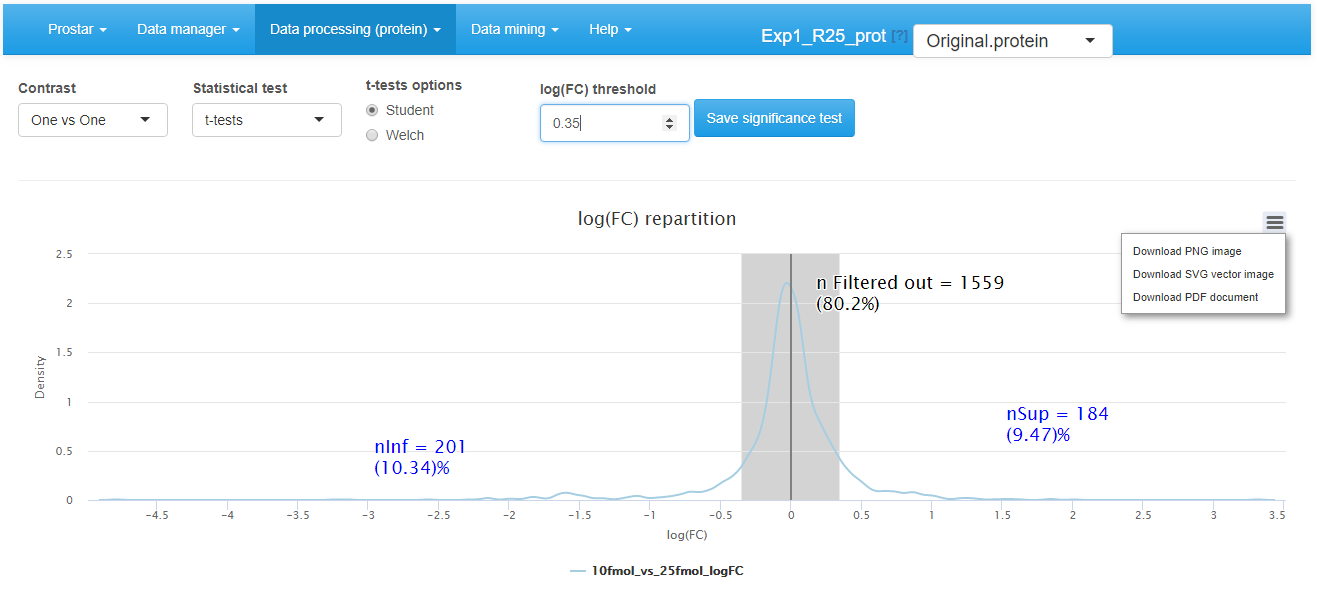
\includegraphics[width=\textwidth]{images/hp.png}
\caption{Hypothesis testing step}
\label{fig:anadiff1}
\end {figure}

First, choose the test contrasts. In case of 2 conditions to compare, there is only one possible contrast. 
However, in case of $N  \geq 3$ conditions, several pairwise contrasts are possible. 
Notably, it is possible to perform $N$ tests of the \textbf{1vsAll} type, or $N(N-1)/2$ tests of the \textbf{1vs1} type.
Then, choose the type of statistical test, between limma (see the \Biocpkg{limma} package) or t-test (either Welch or Student, up to the user's choice). This makes appear a density plot representing the log fold-change (logFC) (as many density curves on the plot as contrasts). Thanks to the FC density plot, tune the \textbf{log(FC) threshold}.
We advise to tune the logFC threshold conservatively by avoiding discarding to many proteins with it. Moreover, it is important tune the logFC to a small enough value, so as to avoid discarding too many proteins. In fact, it is important to keep enough remaining proteins for the next coming FDR computation step (see Section~\ref{sec:pushpval}), as \emph{(i)} FDR estimation is more reliable with many proteins, \emph{(ii)} FDR, which relates to a percentage, does not make sense on too few proteins.
Finally, run the tests and save the dataset to preserve the results (i.e. all the computed p-values). Then, a new dataset containing the p-values and logFC cut-off for the desired contrasts, can be explored in the \textbf{Differential analysis} tab available in the \textbf{Data mining} menu.


%%%%%%%%%%%%%%%%%%%%%%%%%

\section{Data mining}
\subsection{Descriptive statistics}\label{sec:descriptivestatistics}

Several plots are proposed to help the user have a 
quick and as complete as possible overview of the dataset. This menu is 
an essential element for to check that each processing step 
gives the expected result.

\subsubsection{Overview}
This panel simply displays a table summarizing various quantitative elements on the datasets (see Figure~\ref{fig:sdov}).
It roughly amounts to the data summary that is displayed along with each demo dataset (see Section~\ref{sec:demomode}).

\begin {figure}
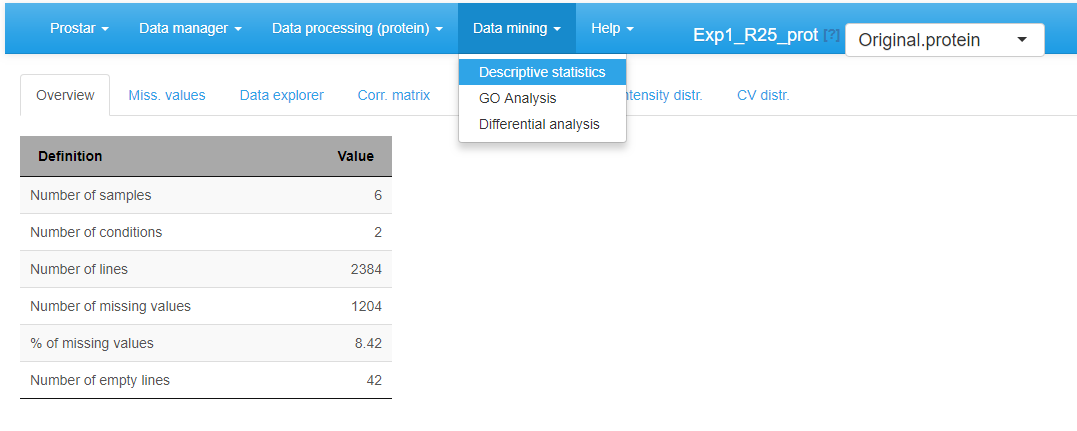
\includegraphics[width=\textwidth]{images/descstat-overview.png}
\caption{Home screen of the Descriptive statistics menu}\label{fig:sdov}
\end {figure}

\subsubsection{Missing values}

On the second tab, barplots depicts the distribution of missing values: the left hand side barplot represents the number of missing values in each sample. The different colors correspond to the different conditions (or groups, or labels). The second barplot (in the middle) displays the distribution of missing values; the red bar represents the empty protein count (i.e. the number of lines in the quantitative data that are only made of missing values). The last barplot represents the same information as the previous one, yet, condition-wise. Let us note that protein with no missing values are represented in the last barplot while not on the second one (to avoid a too large Y-scale).

\begin {figure}
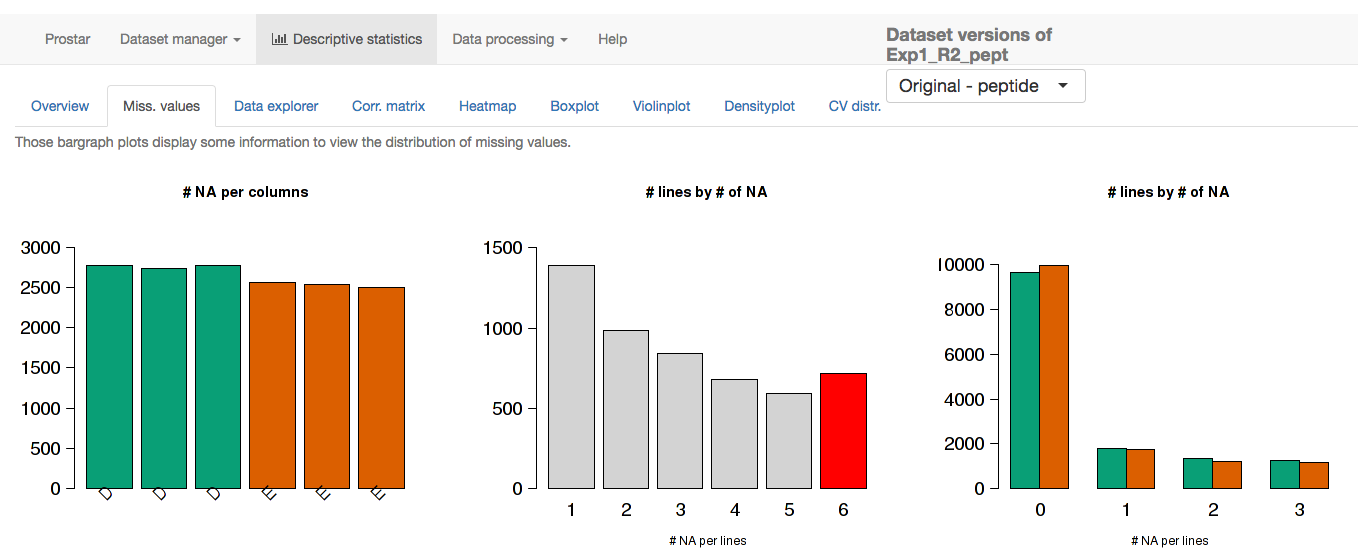
\includegraphics[width=\textwidth]{images/desc_missValues.png}
\caption{Histrograms for the overview of the missing values}\label{fig:sdmv}
\end {figure}

\subsubsection {Data explorer}\label{sec:dataexplorer}
The third tab %is the data explorer (see Figure 4): it 
makes it possible to view the content of the MSnset structure. It is made of three tables, which can be displayed one at a time thanks to the radio button menu. The first one, named \textbf{Quantitative data} contains the intensity values (see Figure~\ref{fig:sdqv1}). 

\begin {figure}
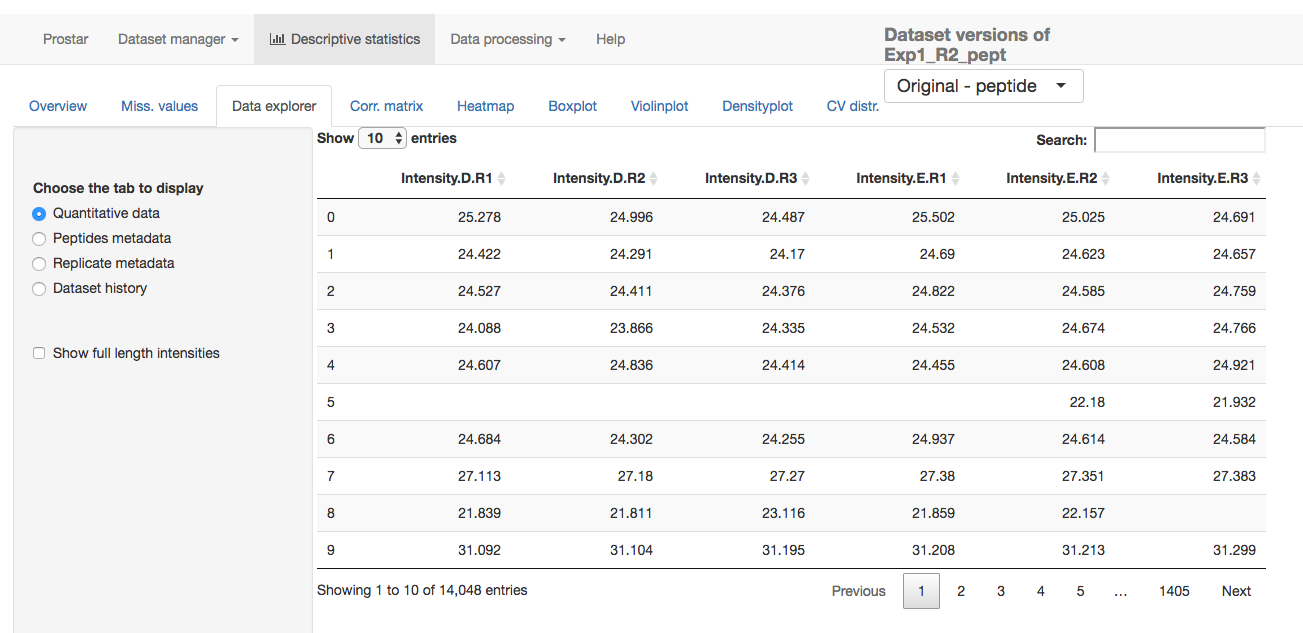
\includegraphics[width=\textwidth]{images/desc_quantiData.png}
\caption{View of quantitative data in the MSnSet dataset}\label{fig:sdqv1}
\end {figure}

The missing values are represented by colored empty cells. The second one is referred to \textbf{Protein metadata}. It contains all the column dataset that are not the quantitative data (see Figure~\ref{fig:sdqv2}). 

\begin {figure}
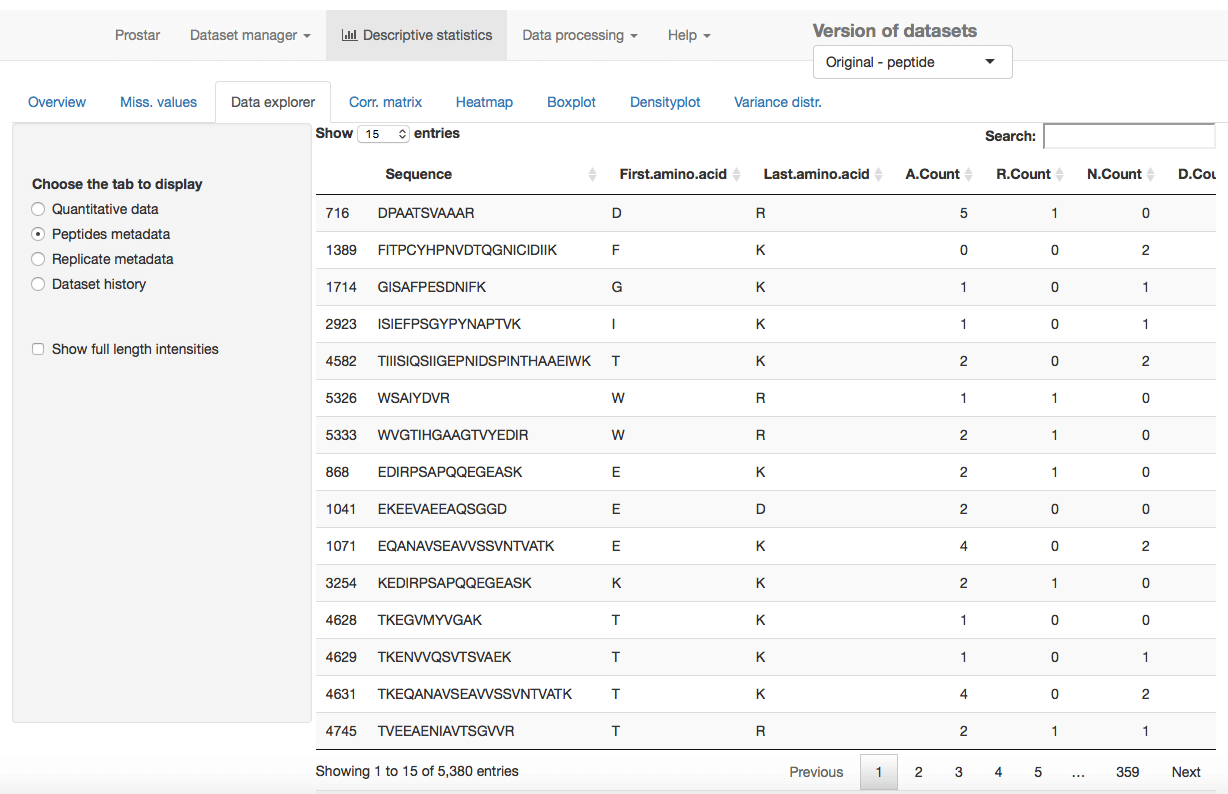
\includegraphics[width=\textwidth]{images/desc_fdata.png}
\caption{View of feature meta-data in the MSnSet dataset}\label{fig:sdqv2}
\end {figure}

The third tab, \textbf{Replicate metadata}, summarizes the experimental design, as defined when converting the data (see Section~\ref{sec:import}). 
%Finally, the last tab, "Dataset history", contains the logs (Note 16) of the previous processing.
%The last tab, named "Dataset history" contains the log of the previous 
%processing. Contrarily to the "Session log" panel (see 
%Section~\ref{sec:sessionlog}), the information here does not relate to the 
%session, and is saved from a session to the next one.

\begin {figure}
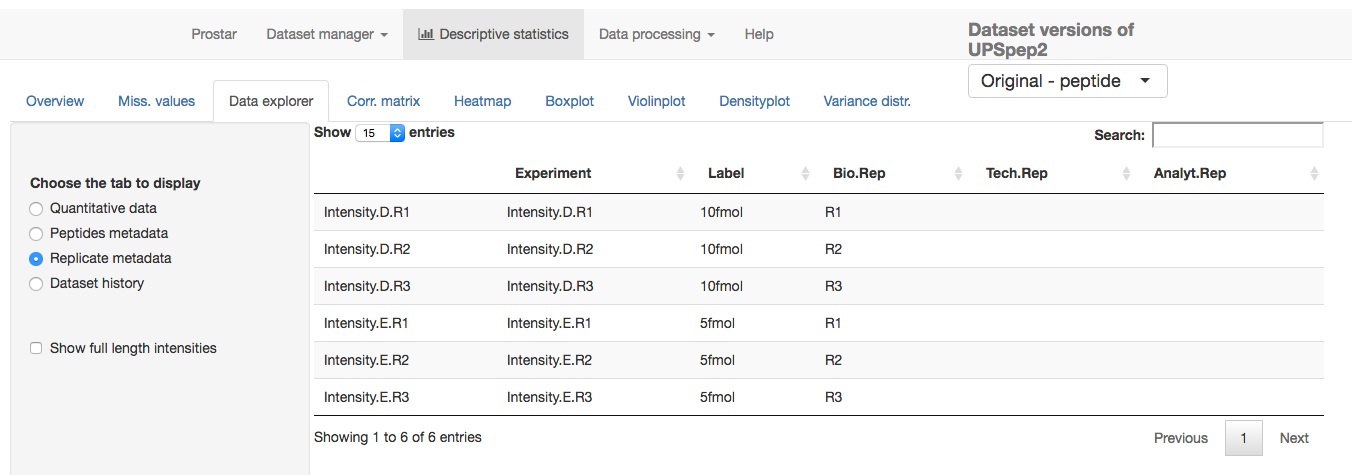
\includegraphics{images/desc_pdata.png}
\caption{View of samples meta-data in the MSnSet dataset}\label{fig:sdqv3}
\end {figure}

\subsubsection {Correlation matrix}

In this tab, it is possible to visualize the extent to which the replicates 
correlate or not (see Figure~\ref{fig:sdcm}). The contrast of the correlation matrix can be tuned thanks to the color scale on the left hand side menu.

\begin {figure}
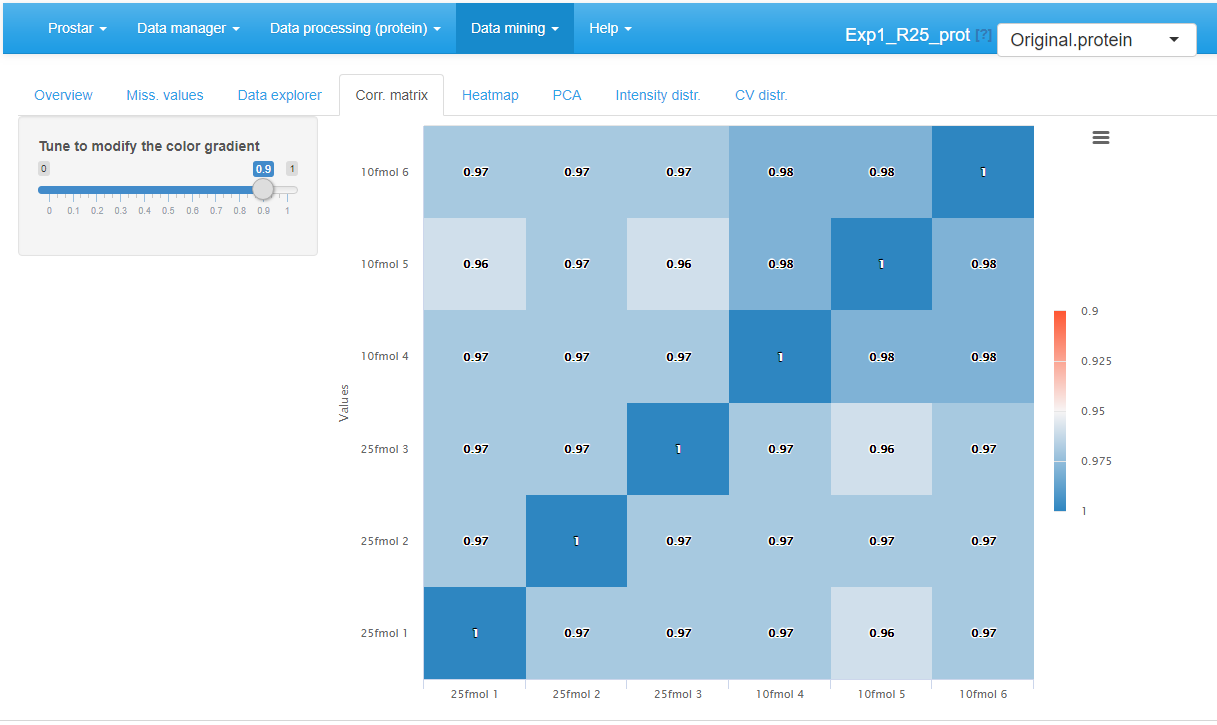
\includegraphics{images/desc_corrmatrix.png}
\caption{Correlation matrix for the quantitative data.}\label{fig:sdcm}
\end {figure}

\subsubsection {Heatmap}
A heatmap as well as the associated dendrogram is depicted on the fifth tab (see Figure~\ref{fig:sdhm}). The colors represent the intensities: red for high intensities and green for low intensities. White color corresponds to missing values. The dendrogram shows a hierarchical classification of the samples, so as to check that samples are related according to the experimental design. It is possible to tune the clustering algorithm\footnote{Computing the heatmap and the dendrogram may be very computationally demanding depending on the dataset.} that produces the dendrogram by adjusting the two parameters of the \Rfunction{hclust} \R{} function:
\begin {itemize}
\item \textbf{Distance}: the parameter method of \Rfunction{stats::dist} function (default is \emph{'euclidean'}).
\item \textbf{Linkage}: the parameter method of \Rfunction{stats::hclust} function (default is \emph{'complete'}).
\end {itemize}

\begin {figure}
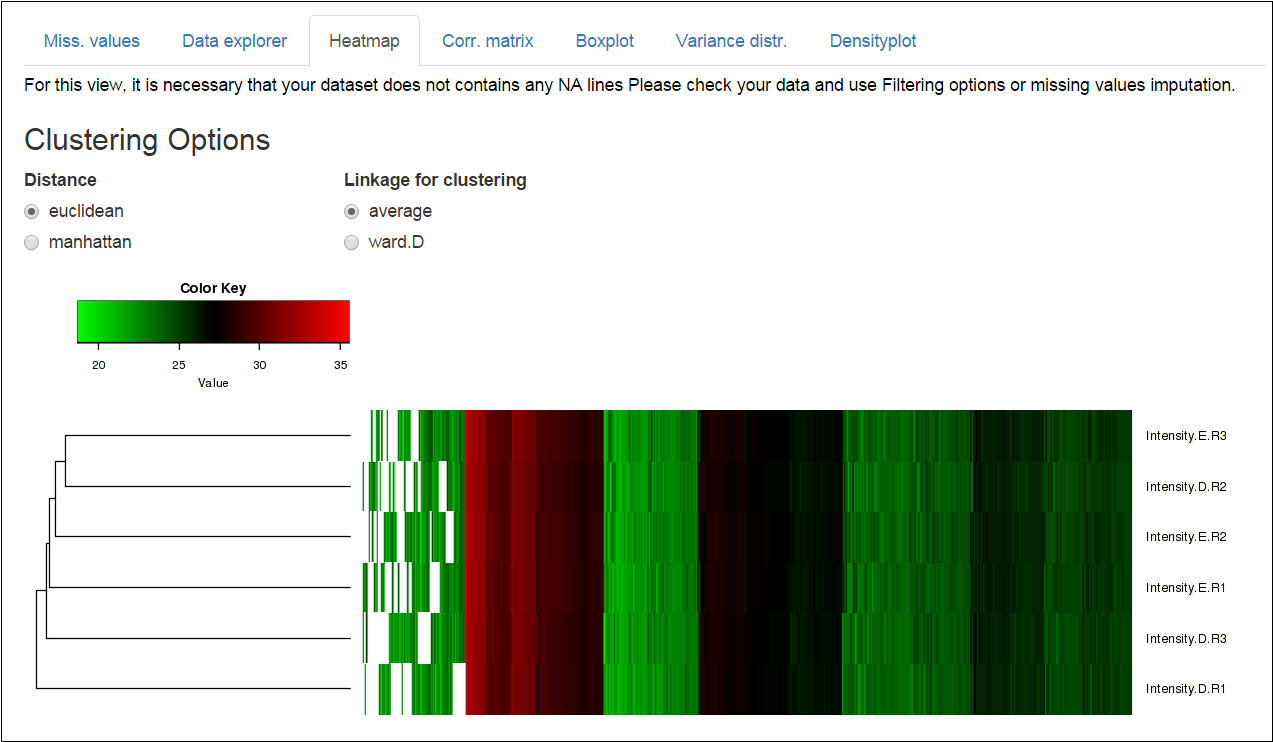
\includegraphics{images/desc_heatmap.png}
\caption{Heatmap and dendrogram for the quantitative data.}\label{fig:sdhm}
\end {figure}

\subsubsection {PCA}\label{sec:pca}

\begin {figure}
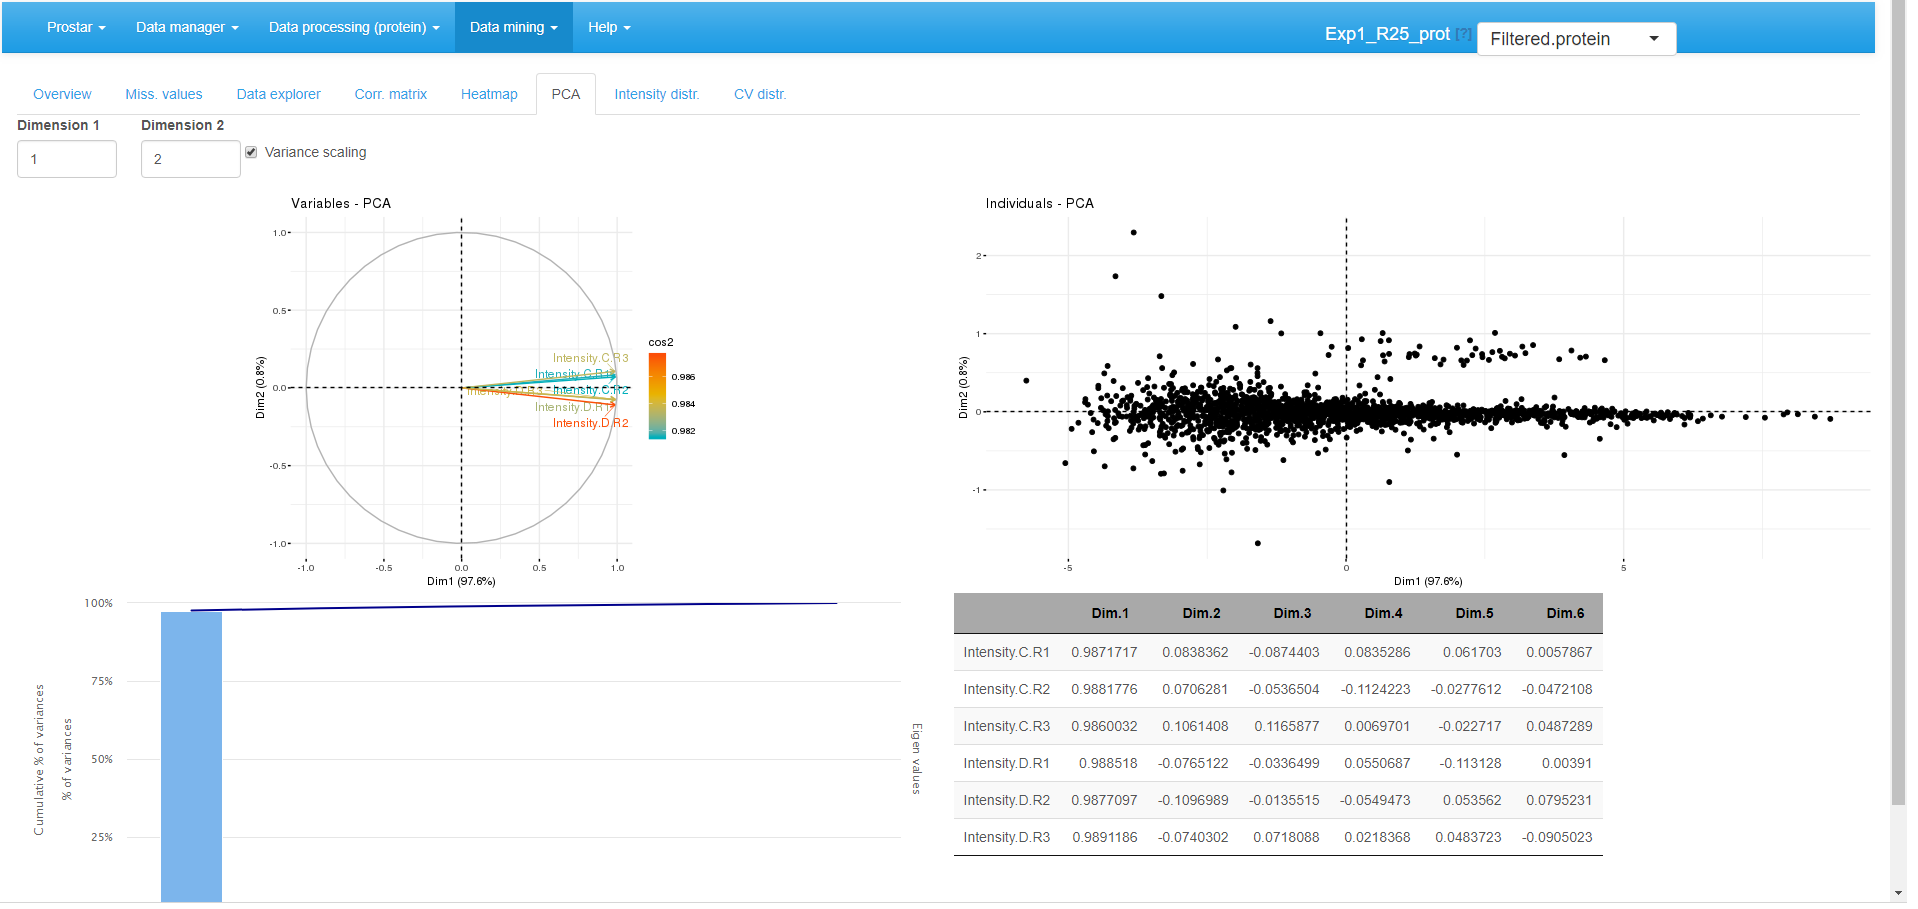
\includegraphics[width=\textwidth]{images/desc_PCA.png}
\caption{Principal compenent analysis tab.}\label{fig:pca}
\end {figure}

A Principal Component Analysis visualization is provided by wrapping the \CRANpkg{FactoMineR} package (see Figure~\ref{fig:pca}). To better interpret the PCA displays, the reader is referred to the \CRANpkg{FactoMineR} documentation. 


\subsubsection {Intensity distributions}\label{sec:densityplot}
These plots shows the distribution of the log-intensity of proteins for each 
condition (see Figure~\ref{fig:sddp}).

The left hand plot represents a smoothed histogram of each sample intensity. The right hand side plot display the same information under the form of a boxplot or a violin plot, depending on the user's choice. In both cases, it is possible to ajust the plot legends, as well as to specify the color code (one color per condition or per sample).

\begin {figure}
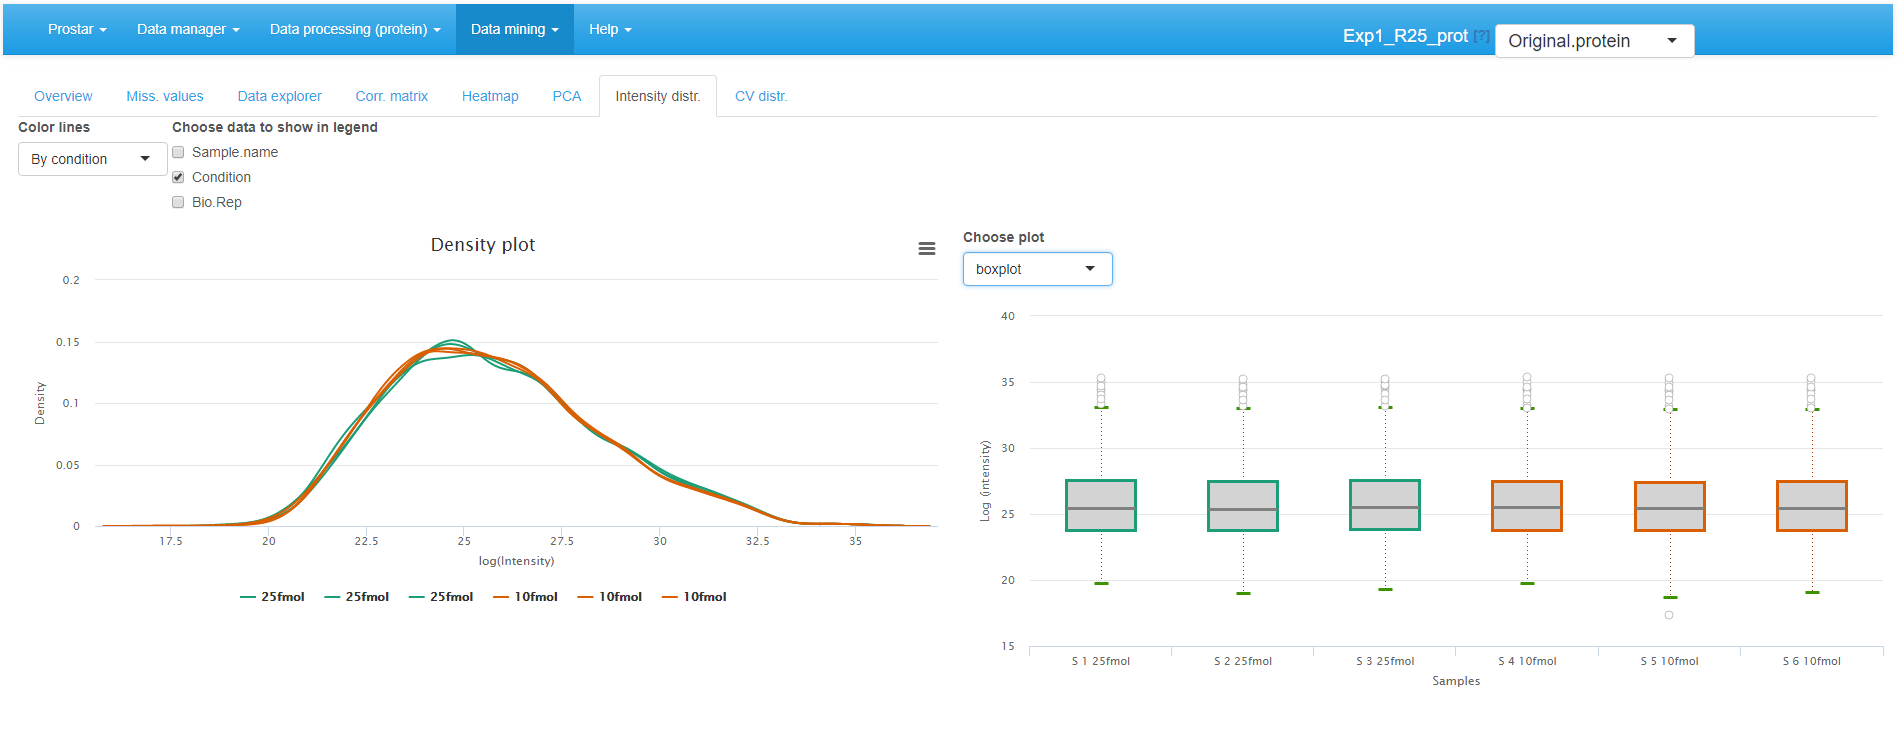
\includegraphics[width=\textwidth]{images/desc_intdistrib.png}
\caption{Densityplot the quantitative data.}\label{fig:sddp}
\end {figure}

%%%%%%%%%%%%%%%%%%%%%%

\subsubsection{CV distribution}

Finally, the last tabs display a density plot of the variance (within each condition) conditionally to the log-intensities  (see Figure~\ref{fig:sdvdZoomOut}).
As is, the plot is often difficult to read, as the high variances are concentrated on the lower intensity values. 
However, it is possible to interactively zoom in on any part of the plot by clicking and dragging (see Figure~\ref{fig:sdvdZoomIn}).

\begin {figure}
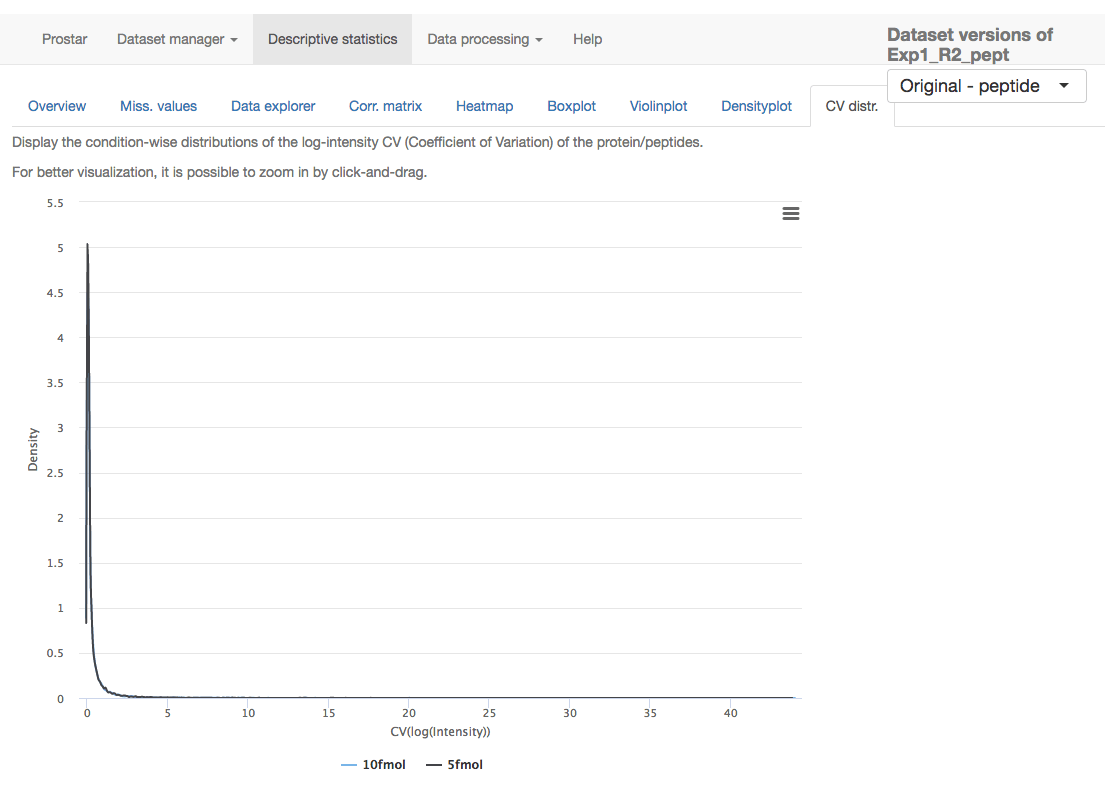
\includegraphics[width=\textwidth]{images/desc_CVDist_ZoomOut.png}
\caption{CV distribution for the quantitative data.}\label{fig:sdvdZoomOut}
\end {figure}

\begin {figure}
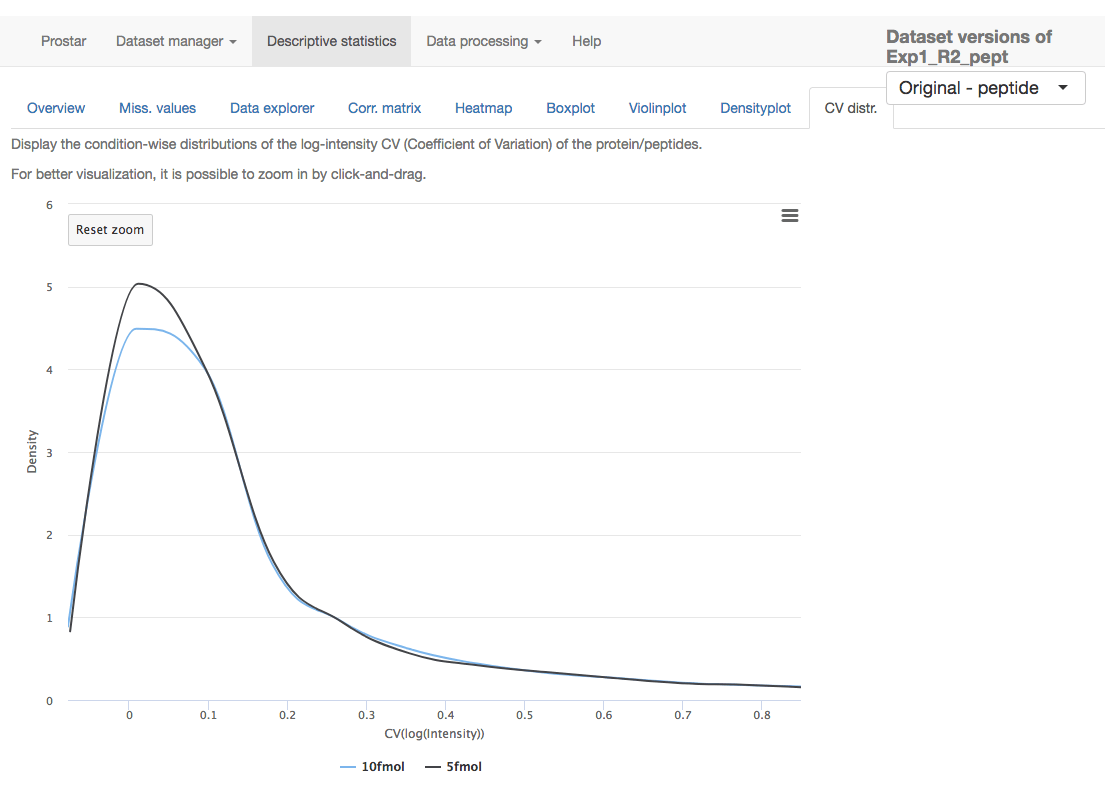
\includegraphics[width=\textwidth]{images/desc_CVDist_ZoomIn.png}
\caption{Zoom in of the CV distribution for the quantitative data.}\label{fig:sdvdZoomIn}
\end {figure}


%%%%%%%%%%%%%%%%%%%%%%%%%%%%%%%%%%%%%%%%%%%%%%%%%%%%%%%%%%%%%%%%%%%
\subsection{Differential analysis}\label{diffana}

If one clicks on \textbf{Differential analysis} in the \textbf{Data mining} menu, it is possible to analyze the protein-level outputs of all statistical tests (see Section~\ref{sec:hp}).
Such analysis follows 5 steps, each corresponding to a separate tab in the \textbf{Differential analysis} menu.

\subsubsection{General methodology}
  
On the first tab, select a pairwise comparison of interest\footnote{In case of a dataset with only 2 different conditions, only one comparison is possible.}. The corresponding volcano plot is displayed. By clicking on a protein in the volcano plot, one or several tables appears below the plot. In any case, a table containing the  intensity values of the protein across the samples is displayed, with the same color code as in the Data explorer (for missing values for instance). In addition, if peptide-level information has been uploaded in the \Biocpkg{Prostar} session, then, the intensity values of the protein can be linked to the original peptides of the dataset. Thus, the peptides intensities (for both protein-specific and shared peptides) are displayed in the 2 other tables.

Possibly, swap the FC axis with the corresponding tick-box, depending on layout preferences. Possibly, push some p-values to 1, as detailed in Section~\ref{sec:pushpval} (see Figure~\ref{fig:pushpval}). 
\begin {figure}
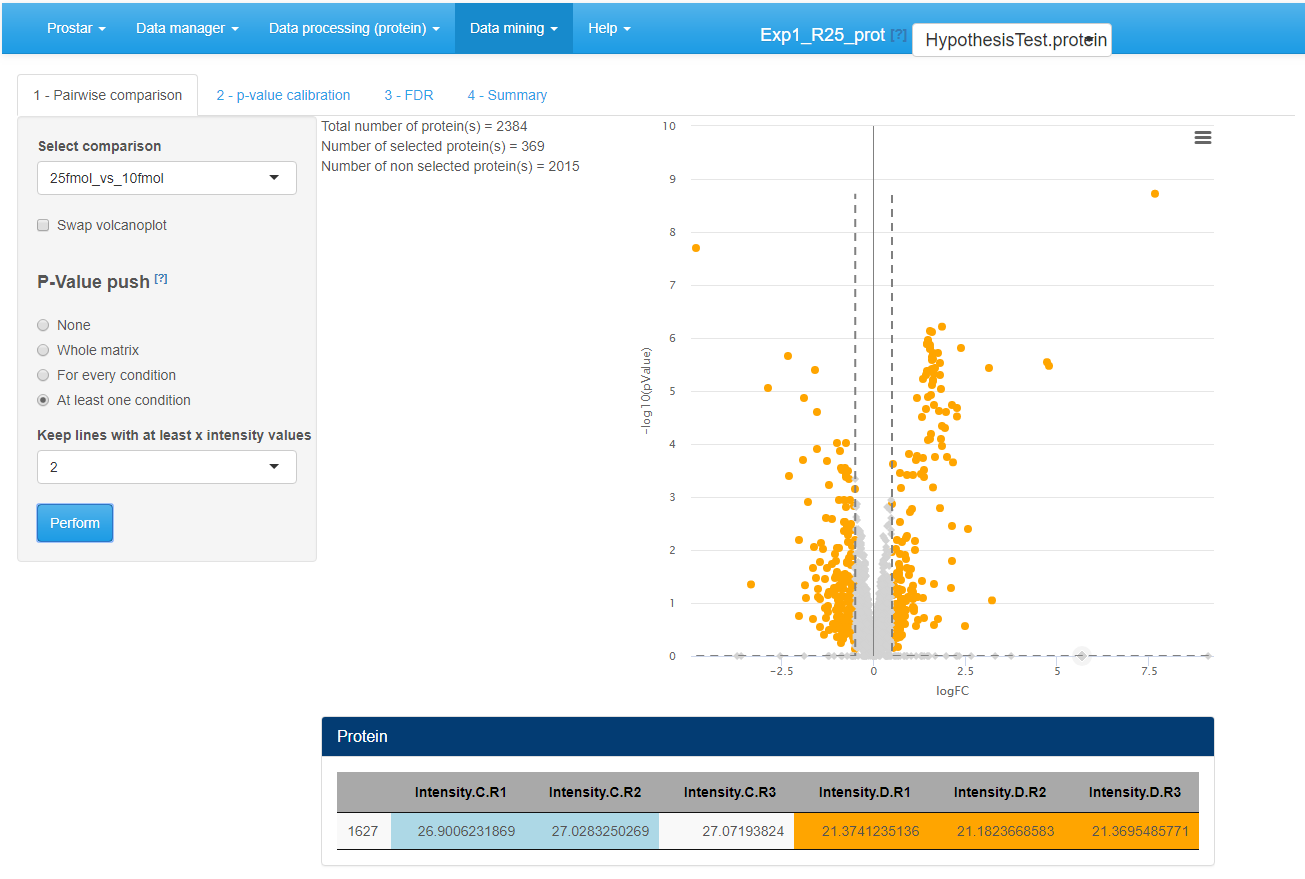
\includegraphics[width=\textwidth]{images/pushpval.png}
\caption{Differential analysis - Tab 1}\label{fig:pushpval}
\end {figure}

Then move on to the next tab, referred to as \textbf{p-value calibration} (see Figure~\ref{fig:cp4p-default}).  
Possibly\footnote{The default tuning of the calibration being the most conservative one, it is possible to skip this step without any risk to spoil the data.}, tune the calibration method, as as detailed in Section~\ref{sec:cp4p}.

\begin {figure}
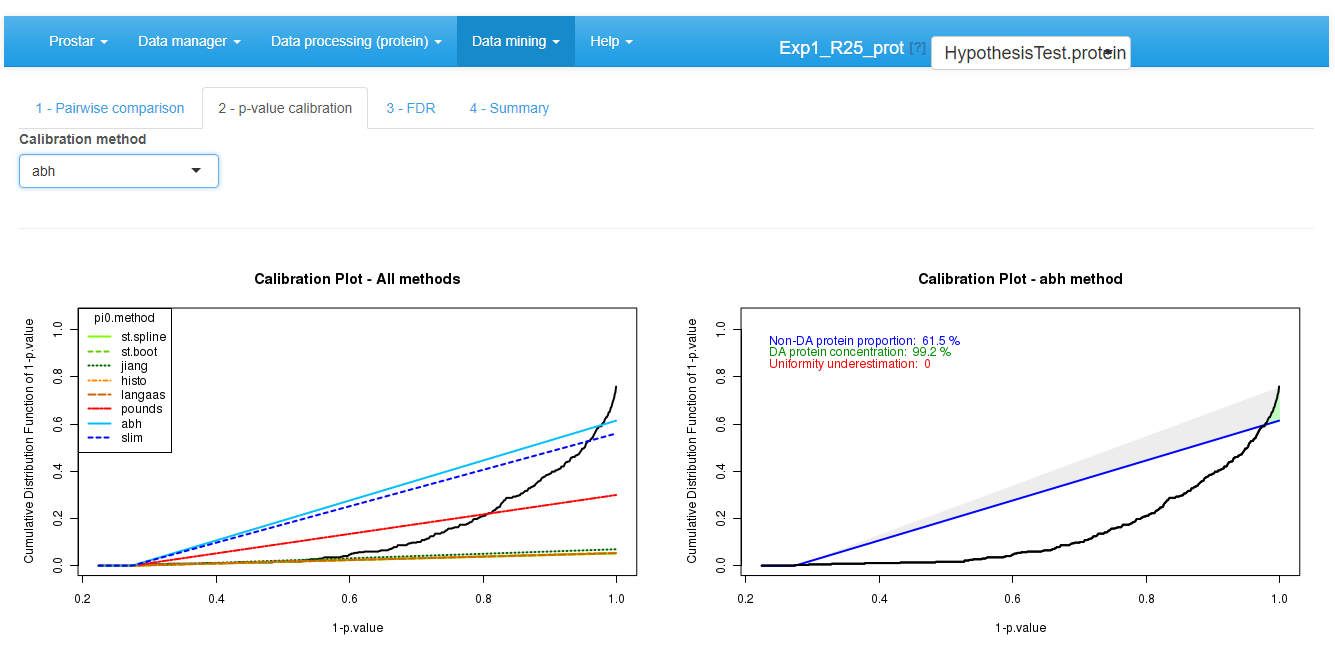
\includegraphics[width=\textwidth]{images/cp4p-default.png}
\caption{Differential analysis - Tab 2}\label{fig:cp4p-default}
\end {figure}

Move on to the next tab and adjust the FDR threshold (see Figure~\ref{fig:fdr-thresh}), which corresponds to the horizontal dashed line on the volcano plot.  The checkbox ``Show p-value table'' displays a table below the volcano plot, where each line represents a protein along with its p-value and logFC. Moreover, it is indicated by a binary variable if, according to the FDR threshold, the protein is deemed differentially abundant or not. For better visualization, this binary variable also encodes the color code applied to each line. The ``Tooltip'' parameter amounts to the list of the avialable meta-data. It is possible to select several of them. The selected one will (1) appear beside the mouse pointer when flying over each protein point in the volcano plot; (2) add the corresponding column in the table below the volcano plot. This table can be easily exported: The user only has to choose whether all the proteins should appear in the exported table, or only the differentially abundant ones. The volcano plot can be saved thanks to the menu available in the upper right corner of the plot.

\begin {figure}
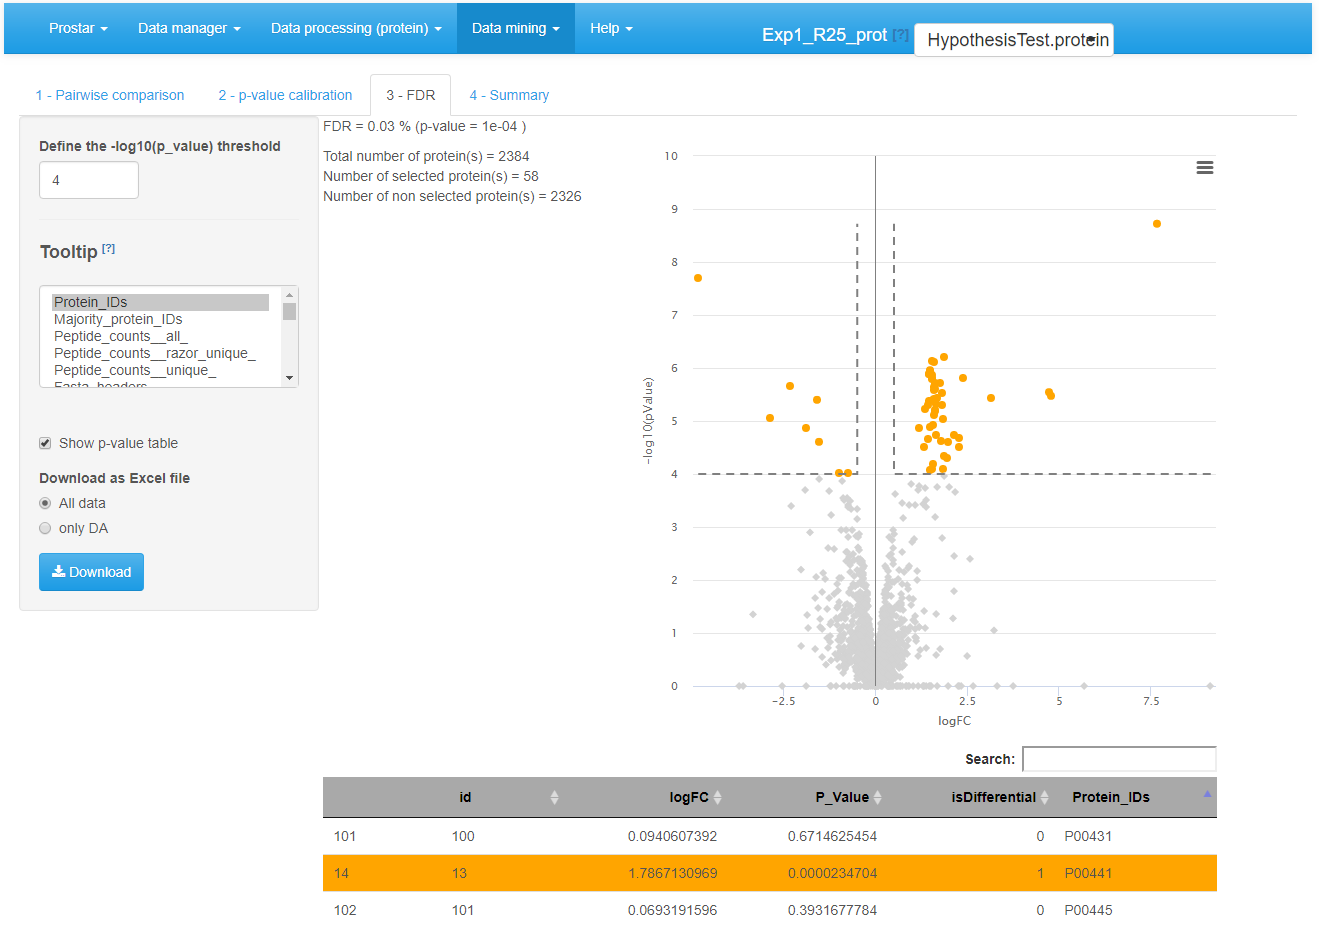
\includegraphics[width=\textwidth]{images/fdr-thresh.png}
\caption{Differential analysis - Tab 3}\label{fig:fdr-thresh}
\end {figure}

Move on to the last tab (referred to as \textbf{Summary}) to have a comprehensive overview of the differential analysis parameters (see Figure~\ref{fig:anadiffsum}). If necessary copy/paste this table for later use.

\begin {figure}
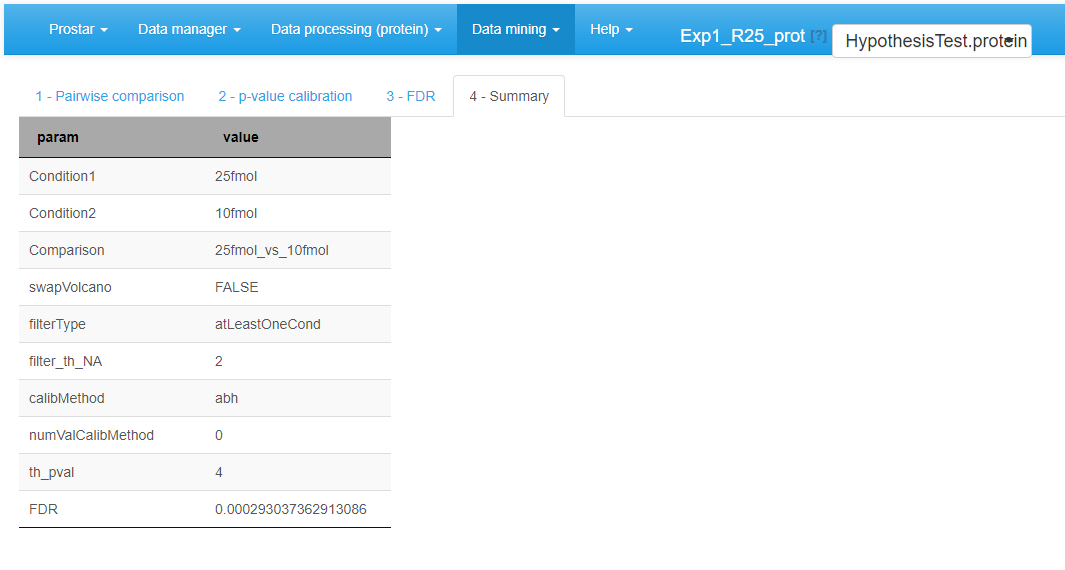
\includegraphics[width=\textwidth]{images/anadiffsum.png}
\caption{Differential analysis - Tab 4}\label{fig:anadiffsum}
\end {figure}

Possibly, go back to the first tab, so as to select another pairwise comparison and process it. Alternatively, it is possible to continue with the current protein list so as to explore the functional profiles of the proteins found statistically differentially abundant between the compared conditions (see Section~\ref{sec:GOAnalysis}).


\subsubsection{Focus on: Push p-values}\label{sec:pushpval}
When working on more than two conditions to compare, the missing value filtering options may be difficult to tune, as a given protein can be well-observed in a group of conditions (with no or few missing values) and largely missing in the remaining conditions. To avoid missing relevant proteins with such a behavior, it is advised to be rather loose at the filtering step (for instance by filtering only proteins that are never seen in the majority of the samples of each condition). %, and to rely on the push p-value option available in the differential analysis.

However, with loose filters, proteins with many missing values are kept in the dataset and are then imputed, so as to present a complete intensity distribution for the differential analysis.
Therefore, when focusing on a specific comparison among the multiple possible ones, it is thus possible to face proteins which have largely been imputed in the two conditions, so that in practice, one analyses the differential abundance of a protein that is probabibly missing in the two conditions. From an analytical viewpoint, such protein must not appears as differentially abundant, even if its p-value is exceptional, for it is too largely based on imputed values that are not trustworthy.

This is why, the push p-value option is proposed: it makes it possible to force the p-values of these proteins to 1, and prevent them to become false discoveries. Concretely, one simply has to tune 
parameters of the menu, which are similar to those of the missing value filtering (Section~\ref{sec:filtering}). However, instead of producing discarding some proteins, it keeps them with a p-value forced to 1 (i.e. a log(p-value) to 0).

As an illustration, Figure~\ref{fig:pushpval} displays a case were all the proteins with less than 2 observed (i.e. not imputed) values within each condition have their p-values pushed to 1. These proteins appear as points on the horizontal axis of the graph. Notably, the snapshot was made when the mouse pointer had clicked on one of these proteins which p-value was pushed (the one with an intensity value between 5.5 and 6). Its intensity values across the samples appears in the table below, where one observes that 5 out of 6 values are colored as POV or MEC (see Section~\ref{sec:imputation}). Clearly, such a protein as very poor mass spectrometry evidence, so that even if the imputed values are of different magnitude (leading to a theoretically appealing p-value), it makes sense to discard it.

\subsubsection{Focus on: Calibration plots}\label{sec:cp4p}

\begin {figure}
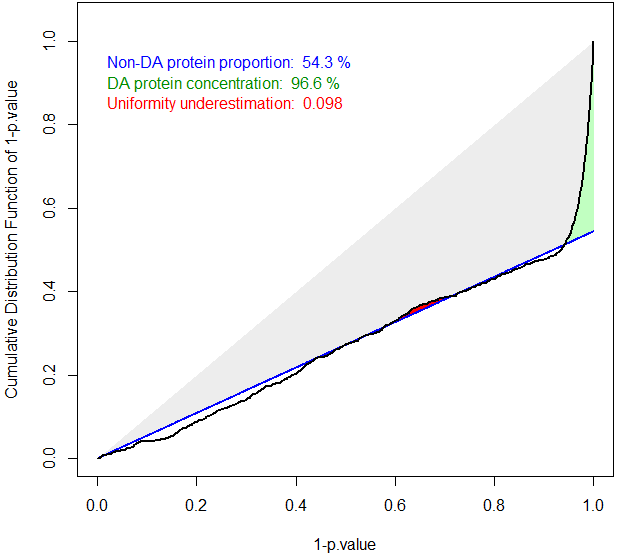
\includegraphics[width=\textwidth]{images/cp4p-ideal.png}
\caption{The ideal case of well calibrated p-values}\label{fig:cp4p-ideal}
\end {figure}

The primary goal of a calibration plot is to check that the p-values have a distribution that is compliant with FDR computation theory.
Given a supposedly known proportion of non-diffentially abundant proteins (generally noted $\pi_0$), a good calibration plot is supposed to depict a curve that follows a straight line of slope $\pi_0$ except for a sharp increase on the right hand side, as depicted on Figure~\ref{fig:cp4p-ideal}. The sharp increase, which is the sign of a good discrimination between proteins which are differentially abundant and those which are not, is depicted in green. On the contrary, any bulb of the curve above the $\pi_0$ line (in blue), anywhere in the middle of the graph is depicted in red, for it is the sign of an insufficient calibration. On Figure~\ref{fig:cp4p-ideal}, the calibration deviation is almost immaterial and the sharpness of the right hand side increase is real: both can be noticed thanks to colored caption (``Uniformity underestimation'' relates to possible red bulps and ``DA protein concentration'' relates to the sharpness of the green region; the last caption, in blue, being $\pi_0$).

\begin {figure}
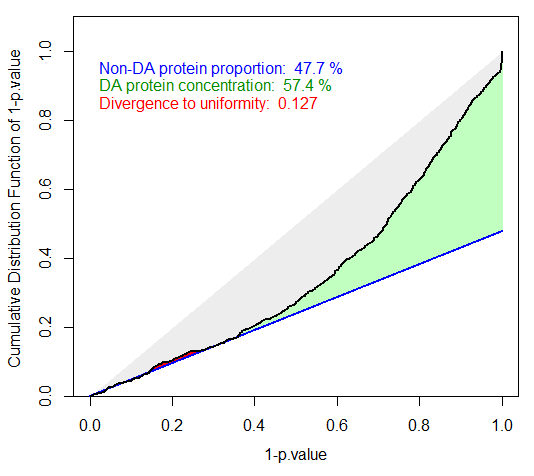
\includegraphics[width=\textwidth]{images/cp4p-pb1.png}
\caption{Badly calibrated p-values, case 1}\label{fig:cp4p-pb1}
\end {figure}


\begin {figure}
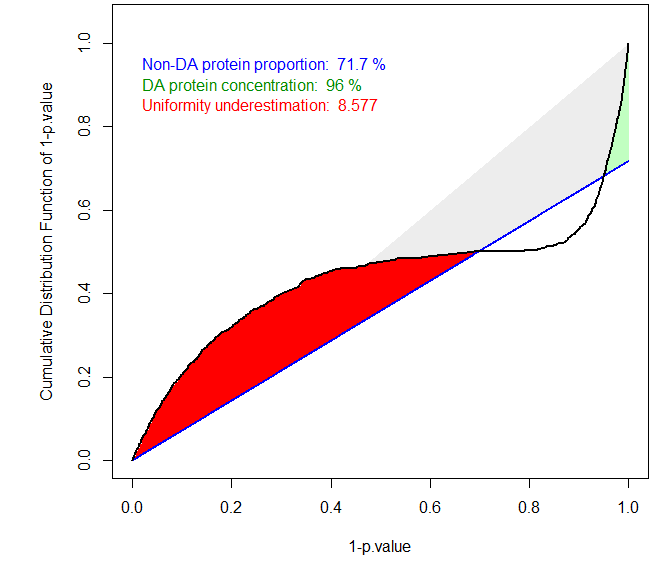
\includegraphics[width=\textwidth]{images/cp4p-pb2.png}
\caption{Badly calibrated p-values, case 2}\label{fig:cp4p-pb2}
\end {figure}

However, it is possible to face situations where the right hand side is not sharp enough (see Figure~\ref{fig:cp4p-pb1}), or where the entire distribution is ill-calibrated (see Figure~\ref{fig:cp4p-pb2}).
In such a cases, FDR computation would lead to spurious values and to biologically irrelevant conclusions. However, if the calibration is not too bad, it is possible to compensate it, by overestimating $\pi_0$. This what the first calibration is made for (see Figure~\ref{fig:cp4p-choice}): several different estimates are depicted by lines of various slope, so as to help the practitioner to choose the most adapted one to the p-value distribution at hand. In the worst case, it is always possible to chose the Benjamini-Hochberg options (corresponding to the safer case of $\pi_0=1$), which is not represented on the graph for it always corresponds to a diagonal line.

\begin {figure}
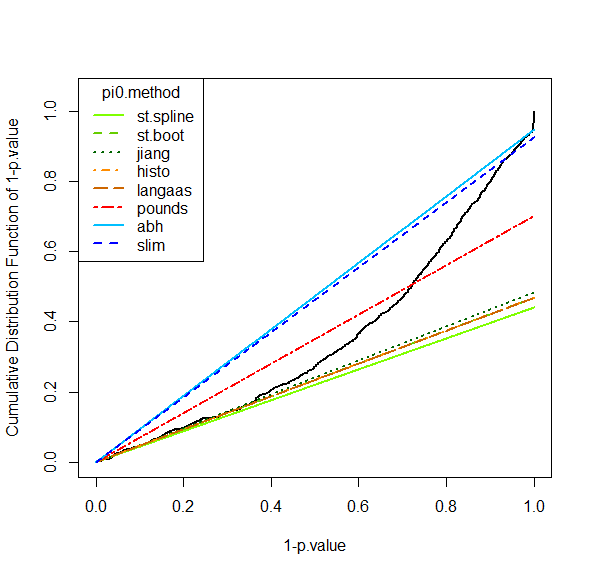
\includegraphics[width=\textwidth]{images/cp4p-choice.png}
\caption{Tuning the $\pi_0$ estimate}\label{fig:cp4p-choice}
\end {figure}

For more details, the interested reader is referred to the \CRANpkg{CP4P} package and the companion publication available in the ``Useful links'' page of \Biocpkg{Prostar} (as well as our tutorial on FDR published by JPR in 2017, also referenced on the same page).


%%%%%%%%%%%%%%%%%%%%%%%%%%%%%%%%%%%%%%%%%%%%%%%%%%%%%%%%%%%%%%%%%%%
\subsection{Gene Ontology analysis}\label{sec:GOAnalysis}

The Gene Ontology (GO, \url{http://www.geneontology.org}) is a controlled vocabulary for
annotating three biological aspects of gene products. This ontology is made of three 
parts : Molecular Function (MF), Biological Process (BP) and Cellular Component 
(CC). 

\textbf{GO analysis} is proposed in the \textbf{Data 
mining} menu. It aims to provide the user with a global view of what is 
impacted (in a biological point of view) in the experiment, by showing which
GO terms are represented (GO classification tab), or over-represented compared 
to a reference (GO enrichment tab). 

\Biocpkg{Prostar} relies on the package \Biocpkg{clusterProfiler} to perform both GO 
Classification and GO Enrichment. We propose a GO analysis interface with
four separated tabs (see Figure~\ref{fig:GO_tab1}): 
    \begin{itemize}
\item GO Setup 
\item GO classification
\item Go Enrichment
\item Parameter summary
\end{itemize}

\begin {figure}

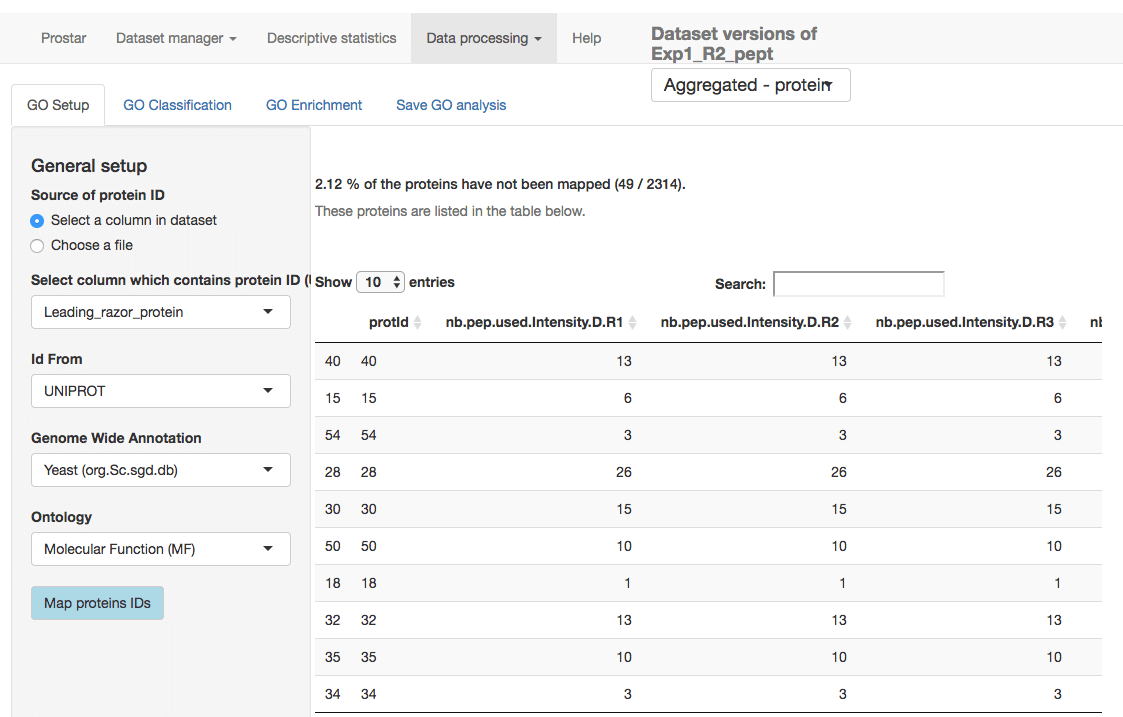
\includegraphics[width=\textwidth]{images/GO_tab1.png}
\caption{GO Setup tab}\label{fig:GO_tab1}
\end {figure}

The left-hand side of the \textbf{GO Setup} tab allows it to set the input parameters, namely: 
\begin{itemize}
\item \textbf{Source of protein ID}: user indicates either a column in the current 
dataset or chooses a file (1 ID per line). 
\item \textbf{Id From}: the type of ID supplied (UNIPROT by default).
\item \textbf{Genome Wide Annotation}: the organism to consider for the analysis.  
\item \textbf{Ontology}: the level of the ontology to work with. 
\end{itemize}

Once these parameters filled, clicking on \textbf{Map proteins IDs} launches the mapping
of the IDs onto the GO categories of the annotation package. 
Then, on the right-hand side of the panel, 
the proportion of proteins that cannot be mapped onto the annotation package
is indicated (this informative ouput does not interrupt the process, unless no 
protein maps). Next step is to perform either GO Classification or GO Enrichment (or both). 

In the \textbf{GO Classification} tab (see Figure~\ref{fig:GO_tab2}), one has to 
indicate which level(s) of the ontology to consider.
Then clicking on the "Perform GO grouping" button launches the analysis 
(function \Rfunction{groupGO()} of the \Biocpkg{clusterProfiler} package). 
The graphics shows the most represented GO categories for a user-defined 
ontology at (a) user-defined level(s).

\begin {figure}
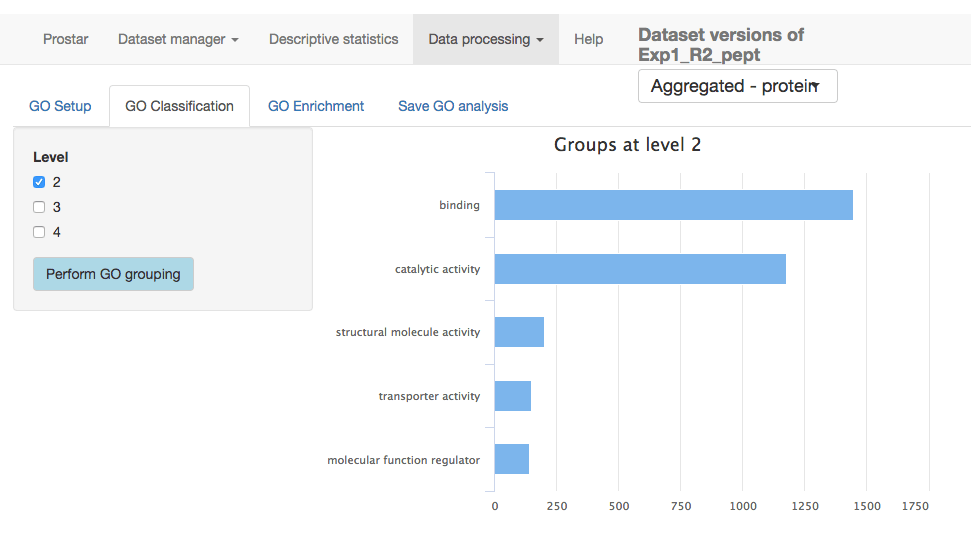
\includegraphics[width=\textwidth]{images/GO_tab2.png}
\caption{GO classification tab}\label{fig:GO_tab2}
\end {figure}

The \textbf{GO Enrichment} tab (see Figure~\ref{fig:GO_tab3}) allows it to know which
GO categories are significantly enriched in the users list, compared 
to a chosen reference ('background' or 'universe'). 
This background can either be : 
\begin{enumerate}
 \item the entire 
organism (in this case, the totality of the proteins identified with an 
"ENTREZGENE" ID in the annotation package specified in the GO Setup tab 
constitutes the background), or 
\item  the entire dataset loaded in Prostar (e.g. all the proteins IDs of the 
'Leading\_razor\_protein' column of the dataset, as illustrated on 
Figure~\ref{fig:GO_tab1}), or 
\item  a custom IDs list provided in a separate file by the user (one ID per line). 
\end{enumerate}


\begin {figure}
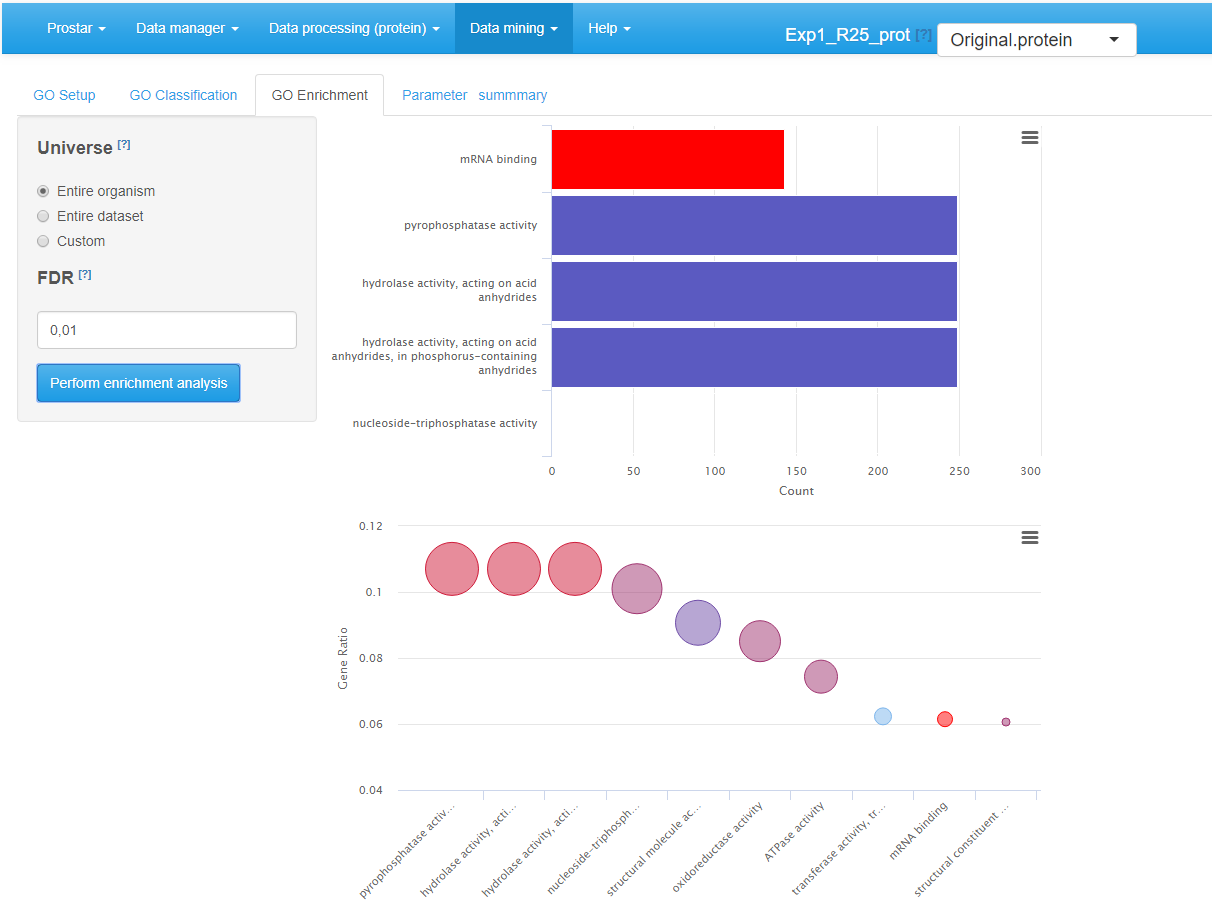
\includegraphics[width=\textwidth]{images/GO_tab3.png}
\caption{GO enrichment tab}\label{fig:GO_tab3}
\end {figure}

The enrichment tab calls the \Rfunction{groupGO()} function of the 
\Biocpkg{clusterProfiler} package. This function performs a significance test
for each category, followed by a multiple test correction at a user-defined level.
Concretely, this level is tuned thanks to 
the "FDR (BH Adjusted $P$-value cutoff)" field. 
Analysis is launched by clicking the \textbf{Perform enrichment analysis} button.

Once the analysis has been performed, the result is displayed via two graphics 
on the right-hand side of the panel (see Figure~\ref{fig:GO_tab3}). 
The first one (top) is a barplot showing the five most significant categories. The 
length of each bar represents the number of proteins within the corresponding category. 
The second one (bottom) is a dotplot ranked by decreasing \textit{GeneRatio}, which reads: 
$$
{\textit{GeneRatio}}
=
\frac{\#(\mbox{Genes of the input list in this category})}
{\#(\mbox{Total number of Genes in the category})}.
$$


The last tab is the \textbf{Save GO analysis} one. It allows saving the results:
GO classification, GO enrichment, or both (see Figure~\ref{fig:GO_tab4}).
Then, a new GOAnalysis dataset is created and loaded in memory. 

As usual in Prostar, it is possible to export this new dataset via the \textbf{Data
manager} menu, either in MSnSet or in Excel format. 

\begin {figure}
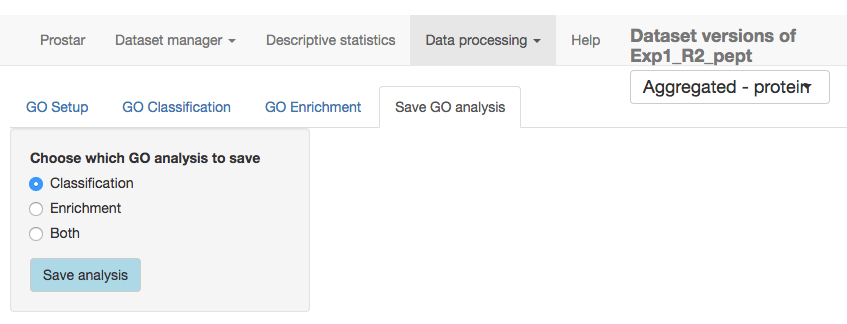
\includegraphics[width=\textwidth]{images/GO_tab4.png}
\caption{GO analysis summary}\label{fig:GO_tab4}
\end {figure}

%\section{Referenced use-cases}
%
%\subsection{Single protein-level pairwise comparison}
%\textbf{\textcolor[rgb]{1,0,0}{XXXX to be completed in release 1.16 XXXX}}
%
%\subsection{Multiple protein-level pairwise comparisons}
%\textbf{\textcolor[rgb]{1,0,0}{XXXX to be completed in release 1.16 XXXX}}
%
%\subsection{Mixed peptide and protein-level comparisons}
%\textbf{\textcolor[rgb]{1,0,0}{XXXX to be completed in release 1.16 XXXX}}
%
%\subsection{Full peptide-level comparisons}
%\fixme[TODO]{missing functionality}
%
%\subsection{Ordered comparisons}
%\fixme[TODO]{missing functionality}
%
%\subsection{Time-course comparisons}
%\fixme[TODO]{missing functionality}
%
%\subsection{Affinity purification comparisons}
%\fixme[TODO]{missing functionality}

%%%%%%%%%%%%%%%%%%%%%%%%%%%%%%%%%%%%%%%%%%%
%% Section
%%%%%%%%%%%%%%%%%%%%%%%%%%%%%%%%%%%%%%%%%%%

\section{Session information}\label{sec:sessionInfo}

\begin{itemize}\raggedright
  \item R version 3.5.1 (2018-07-02), \verb|x86_64-w64-mingw32|
  \item Locale: \verb|LC_COLLATE=French_France.1252|, \verb|LC_CTYPE=French_France.1252|, \verb|LC_MONETARY=French_France.1252|, \verb|LC_NUMERIC=C|, \verb|LC_TIME=French_France.1252|
  \item Running under: \verb|Windows >= 8 x64 (build 9200)|
  \item Matrix products: default
  \item Base packages: base, datasets, graphics, grDevices, methods, parallel, stats, utils
  \item Other packages: Biobase~2.40.0, BiocGenerics~0.26.0, BiocParallel~1.14.2, MSnbase~2.6.4, mzR~2.14.0, Prostar~1.15.0,
    ProtGenerics~1.12.0, Rcpp~0.12.19
  \item Loaded via a namespace (and not attached): affy~1.58.0, affyio~1.50.0, AnnotationDbi~1.42.1, assertthat~0.2.0,
    backports~1.1.2, bindr~0.1.1, bindrcpp~0.2.2, BiocInstaller~1.32.1, BiocManager~1.30.4, bit~1.1-14, bit64~0.9-7,
    bitops~1.0-6, blob~1.1.1, broom~0.5.0, Cairo~1.5-9, caTools~1.17.1.1, cellranger~1.1.0, cluster~2.0.7-1,
    clusterProfiler~3.8.1, codetools~0.2-15, colorspace~1.3-2, colourpicker~1.0, compiler~3.5.1, cowplot~0.9.3, cp4p~0.3.5,
    crayon~1.3.4, curl~3.2, DAPAR~1.15.0, DAPARdata~1.11.2, data.table~1.11.8, DBI~1.0.0, digest~0.6.18, DO.db~2.9,
    doParallel~1.0.14, DOSE~3.6.1, dplyr~0.7.8, DT~0.5, enrichplot~1.0.2, factoextra~1.0.5, FactoMineR~1.41, farver~1.0,
    fastmatch~1.1-0, fgsea~1.6.0, flashClust~1.01-2, forcats~0.3.0, foreach~1.4.4, future~1.10.0, gdata~2.18.0, geeM~0.10.1,
    geepack~1.2-1, ggforce~0.1.3, ggplot2~3.1.0, ggraph~1.0.2, ggrepel~0.8.0, ggridges~0.5.1, globals~0.12.4, glue~1.3.0,
    gmm~1.6-2, GO.db~3.6.0, GOSemSim~2.6.2, gplots~3.0.1, graph~1.58.2, grid~3.5.1, gridExtra~2.3, gtable~0.2.0,
    gtools~3.8.1, haven~1.1.2, highcharter~0.6.0, hms~0.4.2, htmltools~0.3.6, htmlwidgets~1.3, httpuv~1.4.5, httr~1.3.1,
    igraph~1.2.2, imp4p~0.7, impute~1.54.0, IRanges~2.14.12, Iso~0.0-17, iterators~1.0.10, jsonlite~1.5, KernSmooth~2.23-15,
    knitr~1.20, later~0.7.5, lattice~0.20-38, lazyeval~0.2.1, leaps~3.0, limma~3.36.5, listenv~0.7.0, lubridate~1.7.4,
    magrittr~1.5, MALDIquant~1.18, MASS~7.3-51.1, Matrix~1.2-15, memoise~1.1.0, MESS~0.5.2, mime~0.6, miniUI~0.1.1.1,
    modelr~0.1.2, multtest~2.36.0, munsell~0.5.0, mvtnorm~1.0-8, mzID~1.18.0, nlme~3.1-137, norm~1.0-9.5, openxlsx~4.1.0,
    pcaMethods~1.72.0, pillar~1.3.0, pkgconfig~2.0.2, plyr~1.8.4, png~0.1-7, preprocessCore~1.42.0, promises~1.0.1,
    purrr~0.2.5, quantmod~0.4-13, qvalue~2.12.0, R.methodsS3~1.7.1, R.oo~1.22.0, R.utils~2.7.0, R6~2.3.0, rclipboard~0.1,
    RColorBrewer~1.1-2, readr~1.1.1, readxl~1.1.0, reshape2~1.4.3, rhandsontable~0.3.6, rlang~0.3.0.1, rlist~0.4.6.1,
    RSQLite~2.1.1, rstudioapi~0.8, rvcheck~0.1.1, rvest~0.3.2, S4Vectors~0.18.3, sandwich~2.5-0, scales~1.0.0,
    scatterplot3d~0.3-41, shiny~1.2.0, shinyAce~0.3.2, shinyBS~0.61, shinycssloaders~0.2.0, shinyjqui~0.3.2, shinyjs~1.0,
    shinythemes~1.1.2, shinyTree~0.2.6, shinyWidgets~0.4.4, siggenes~1.54.0, splines~3.5.1, stats4~3.5.1, stringi~1.2.4,
    stringr~1.3.1, survival~2.43-1, tibble~1.4.2, tidyr~0.8.2, tidyselect~0.2.5, tidyverse~1.2.1, tmvtnorm~1.4-10,
    tools~3.5.1, truncnorm~1.0-8, TTR~0.23-4, tweenr~1.0.0, units~0.6-1, UpSetR~1.3.3, vioplot~0.2, viridis~0.5.1,
    viridisLite~0.3.0, vsn~3.48.1, webshot~0.5.1, whisker~0.3-2, XML~3.98-1.16, xml2~1.2.0, xtable~1.8-3, xts~0.11-2,
    yaml~2.2.0, zip~1.0.0, zlibbioc~1.26.0, zoo~1.8-4
\end{itemize}
%\bibliography{\Biocpkg{Prostar}}


\end{document}
